\chapter{Probabilistic Circuits}
\label{ch:pc}

As we briefly mentioned in the last chapter, Probabilistic Circuits (PCs) are conceptualized as
computational graphs under special conditions. In this chapter, \Cref{sec:pc} to be more precise,
we formally define PCs and give an intuition on their syntax, viewing other probabilistic models
through the lenses of the PC framework, formalizing the many structural constraints that give
sufficient conditions for tractable inference. In \Cref{sec:pckb}, we address PCs as knowledge
bases, representing logic formulae through circuits.

\section{Distributions as Computational Graphs}
\label{sec:pc}

Probabilistic circuits are annotated computational graphs usually recursively defined in terms of
their computational units. We start with a broad definition of probabilistic circuits.

\begin{definition}[Probabilistic circuit]
  A \emph{probabilistic circuit} $\mathcal{C}$ is a rooted connected annotated DAG whose nodes
  compute tractable operations of their children, usually either convex combinations, known as
  \emph{sum} nodes, or \emph{products}. Nodes with no outgoing edges, i.e.\ \emph{input} nodes, are
  real-valued nonnegative functions with tractable evaluation and marginalization. Computing a
  value from $\mathcal{C}$ amounts to a bottom-up pass from input nodes to root. \label{def:pc}
\end{definition}

In its simplest form, a PC is a single input node representing any tractable unnormalized
probability density. More concretely, inputs are typically parametric univariate density (or mass)
functions, although joint probability density functions of complex non-parametric models are
supported as well. To simplify notation, from here on out we shall use the term distribution to
mean a probability density (or mass) function and argue that input nodes represent probability
distributions. The semantics of this shall be clear given the context.

Let $\Leaf_p$ a PC input node representing a distribution $p$ and an assignment $\set{x}$ of random
variables $\set{X}$; we use the notation $\Leaf_p(\set{X}=\set{x})$ to mean $p(\set{X}=\set{x})$,
often omitting $p$ when its explicit form is not needed and $\set{X}$ when meaning is clear from
context. We say that the scope of $\Leaf_p$, denoted by $\Sc(\Leaf_p)$, is the set of all random
variables that come into play in the probability distribution $p$. When $\set{x}$ captures the
entire scope of a node, i.e.\ $\set{x}$ assigns a value to every variable $X\in\Sc(\Node)$, it is
said to be a \emph{complete assignment}, or a \emph{partial assignment} otherwise. When we say that
an input node must be \emph{tractable}, we mean that it must \emph{at worst} be able to compute the
\emph{probability evidence} and \emph{marginal probability} of any assignment $\set{x}$ in
polynomial time. We define probability of evidence as a complete assignment $\set{x}$'s likelihood
according to the probabilistic circuit, while the marginal probability is the marginalization of a
partial assignment's remaining random variables $\set{Y}$:
$\int_{\set{y}}p(\set{x},\set{y})\dif\set{y}$. The value, be it the probability of evidence or
marginal probability, of an input node is the same of the distribution it represents under a given
evidence. We abuse notation and say that $\Leaf_p(\set{x})=\int_{\set{y}}p(\set{x},
\set{y})\dif\set{y}$ is the marginal of partial assignment $\set{x}$. To facilitate analysis, we
assume that evaluating any query on an input node is node in $\bigo(1)$. \Cref{eg:gaussians} shows
an instance of a Gaussian distribution as a PC.

\begin{example}[sidebyside,lefthand width=0.6\textwidth]{Gaussians as probabilistic circuits}{gaussians} %
  Let $\mathcal{C}$ a probabilistic circuit with a single (input) node $\Leaf$. We associate
  $\Leaf$ with a univariate Gaussian distribution $p(X)=\gaussian(X;\mu,\sigma^2)$, meaning that
  any query on $\Leaf$ directly translates to $p$. As an example, suppose $\mu=0$ and $\sigma^2=1$
  and we wish to compute $\Leaf(x=0.8;\mu,\sigma^2)$. The probability of this input shall then be
  \begin{equation*}
    \Leaf(x=0.8;\mu,\sigma^2)=\gaussian(x=0.8;\mu=0,\sigma^2=1)=0.29.
  \end{equation*}
  Likewise, the marginal probability of a random variable $Y$ not in $\Sc(L)=\{X\}$ for the
  probabilistic circuit $\mathcal{C}$ rooted at $\Leaf$ is the marginal of $p$
  \begin{equation*}
    \Leaf(y;\mu,\sigma^2)=\int_x\Leaf(x,y;\mu,\sigma^2)\dif{}x=1.0.
  \end{equation*}
  \tcblower
  \centering
  \begin{tikzpicture}
    \pgfplotsset{
      every axis/.append style={
        axis line style={->},
        tick label style={font={\scriptsize\bfseries}},
        x tick label style={color=white,above right},
        y tick label style={color=white,above right},
        grid style={black,dashed},
      }
    }
    \begin{axis}[
      no markers, domain=-5:5, samples=35,
      height=2.75cm, width=\columnwidth,
      xtick={0.8}, ytick={0.29},
      xticklabels={\colorbox{boxblue}{\textbf{0.8}}},
      yticklabels={\colorbox{boxgreen}{\textbf{0.29}}},
      axis lines*=left, xlabel=$x$, ylabel=$p(x)$,
      every axis y label/.style={font=\scriptsize,at={(axis description cs:-0.1,0.9)},anchor=south},
      every axis x label/.style={font=\scriptsize,at=(current axis.right of origin),anchor=west},
      enlargelimits=false, clip=false, axis on top,
      grid = major
    ]
      \addplot[very thick,boxteal] {gauss(0,1)};
    \end{axis}
  \end{tikzpicture}

  \begin{tikzpicture}
    \node (x) at (0, 0) {$x$};
    \newGaussNode{g}{$(x) + (1,0)$};
    \node (px) at ($(g) + (1.25,0)$) {$p(x)$};
    \draw[boxdgray,edge] (x) -- (g);
    \draw[boxdgray,edge] (g) -- (px);

    \newGaussNode[label=below:$X$]{gv}{$(g) - (0,1.0)$};
    \node (xv) at ($(gv) - (1.25,0)$) {\colorbox{boxblue}{\color{white}$\mathbf{.80}$}};
    \node (pxv) at ($(gv) + (1.25,0)$) {\colorbox{boxgreen}{\color{white}$\mathbf{.29}$}};
    \draw[boxdgray,edge] (xv) -- (gv);
    \draw[boxdgray,edge] (gv) -- (pxv);
  \end{tikzpicture}

  \begin{tikzpicture}
    \pgfplotsset{
      every axis/.append style={
        axis line style={->},
        tick label style={},
        grid style={black}
      }
    }
    \begin{axis}[
      no markers, domain=-5:5, samples=35,
      xtick={-5}, ytick={0},
      xticklabels={}, yticklabels = {},
      height=2.75cm, width=\columnwidth,
      axis lines*=left, xlabel=$x$, ylabel=$p(x)$,
      every axis y label/.style={font=\scriptsize,at={(axis description cs:-0.1,0.9)},anchor=south},
      every axis x label/.style={font=\scriptsize,at=(current axis.right of origin),anchor=west},
      enlargelimits=false, clip=false, axis on top,
      grid=major
    ]
      \path[name path=axis] (axis cs:0,0) -- (axis cs:5,0);
      \addplot[very thick,boxteal,name path=g] {gauss(0,1)};
      \addplot[boxteal!80] fill between [of=g and axis];
      \node at (2.5,0.3) {\colorbox{boxblue}{\color{white}\scriptsize\textbf{1.0}}};
    \end{axis}
  \end{tikzpicture}
\end{example}

An inner node indicates an operation to be computed from the value of its children. The subject of
which operations yield which benefits in terms of inference is an interesting question which we
briefly touch in \Cref{rem:optract}, but otherwise remains out of the scope of this work. In this
dissertation, we restrict ourselves to the study of \emph{sums} and \emph{products}. We first
address sums, which appear as convex combinations in probabilistic circuits.

Let $\Sum$ be a PC sum node, and denote by $\Ch(\Sum)$ the child nodes of $\Sum$. For every edge
$\edge{\Sum\Child}$ coming out of $\Sum$ and going into $\Child$, we attribute a weight $w_{\Sum,
\Child}\geq 0$, such that $\sum_{\Child\in\Ch(\Sum)} w_{\Sum,\Child} = 1$. A sum node semantically
defines a mixture model over its children, essentially acting as a latent variable over the
component distributions \citep{poon11,peharz16}. Its value is the weighted sum of its children
$p_{\Sum}(\set{x})=\sum_{\Child\in\Ch(\Sum)}w_{\Sum,\Child}\cdot p_{\Child}(\set{x})$. Again, to
simplify notation we shall use $\Node(\set{x})$ as an alias for $p_{\Node}(\set{x})$, that is, the
probability distribution given by a node $\Node$'s induced distribution. \Cref{eg:mixgauss} shows a
case of a Gaussian mixture model as a PC.

So far, the only nonlinearities present in PCs come from the internal computations of input nodes.
In fact, a PC that only contains sums and inputs can always be reduced to a mixture model (see
\Cref{thm:summix}). Adding \emph{product nodes} as another form of nonlinearity increases
expressivity sufficiently for PCs to be capable of representing any discrete probability
distribution \citep{darwiche03,martens14,peharz15}. More importantly, products semantically act as
factorizations of their children, indicating a conditional independence relationship between
variables from different children given the value of a latent variable. In practice, product nodes
are simply products of their children: if $\Prod$ is a PC product node, then its value is given by
$\Prod(\set{x})=\prod_{\Child\in\Ch(\Prod)} \Child(\set{x})$.

\newcommand\mone{1}%
\newcommand\sone{0.65}%
\newcommand\mtwo{2.5}%
\newcommand\stwo{0.85}%
\newcommand\mthr{4}%
\newcommand\sthr{0.6}%
\begin{example}[sidebyside,lefthand width=0.55\textwidth]{Gaussian mixture models as probabilistic circuits}{mixgauss}
  A Gaussian Mixture Model (GMM) defines a mixture over Gaussian components. Say we wish to compute
  the probability of $X=x$ for a GMM $\mathcal{G}$ with three components
  $\gaussian_1(\mu_1=\mone,\sigma^2_1=\sone)$, $\gaussian_2(\mu_2=\mtwo, \sigma^2_1=\stwo)$ and
  $\gaussian_3(\mu_3=\mthr,\sigma^2_3=\sthr)$, and suppose we have weights set to
  $\phi=(0.4,0.25,0.35)$. Computing the probability of $x$ according to $G$ amounts to the weighted
  summation
  \begin{align*}
    \mathcal{G}(X=x)=&0.4\cdot\gaussian_1(x;\mu_1,\sigma^2_2)+0.25\cdot\gaussian_2(x;\mu_2,\sigma^2_2)+\\
                     &0.35\cdot\gaussian_3(x;\mu_3,\sigma^2_3),
  \end{align*}
  which is equivalent to a computational graph (i.e. a PC) with a sum node whose weights are set to
  $\phi$ and children are the components of the mixture. The figure on the right shows
  $\mathcal{G}$ (top) and its corresponding PC (middle). Given $x=1.5$ (in blue), input nodes are
  computed following the inference flow (bottom, gray edges) up to the root sum node (in red),
  where a weighted summation is computed to output the probability (in green).

  \tcblower
  \begin{center}
    \begin{tikzpicture}
      \pgfplotsset{
        every axis/.append style={
          axis line style={->},
          tick label style={font={\scriptsize\bfseries}},
          x tick label style={color=white,below},
          y tick label style={color=white,left},
          grid style={black,dashed},
        }
      }
      \begin{axis}[
        no markers, domain=-1:6, samples=35,
        height=3.75cm, width=\columnwidth,
        xtick={1.5}, ytick={0.2414},
        xticklabels={\colorbox{boxblue}{\textbf{1.5}}},
        yticklabels={\colorbox{boxgreen}{\textbf{0.24}}},
        axis lines*=left, xlabel=$x$, ylabel=$p(x)$,
        every axis y label/.style={font=\scriptsize,at={(axis description cs:-0.1,0.9)},anchor=south},
        every axis x label/.style={font=\scriptsize,at=(current axis.right of origin),anchor=west},
        enlargelimits=false, clip=false, axis on top,
        grid = major
      ]
        \path[name path=axis] (axis cs:0,0) -- (axis cs:5,0);
        \addplot[very thick,boxteal,name path=g1] {gauss(\mone,\sone)};
        \addplot[very thick,boxorange,name path=g2] {gauss(\mtwo,\stwo)};
        \addplot[very thick,boxpurple,name path=g3] {gauss(\mthr,\sthr)};
        \addplot[very thick,boxred] {mixgauss3(\mone,\sone,\mtwo,\stwo,\mthr,\sthr,0.4,0.25,0.35)};
        \addplot[boxteal!60] fill between [of=g1 and axis];
        \addplot[boxorange!50] fill between [of=g2 and axis];
        \addplot[boxpurple!40] fill between [of=g3 and axis];
        \node at (\mone, 0.7) {\tiny$\mu_1=\mone$};
        \node at (\mtwo, 0.5) {\tiny$\mu_2=\mtwo$};
        \node at (\mthr, 0.75) {\tiny$\mu_3=\mthr$};
      \end{axis}
    \end{tikzpicture}

    \begin{tikzpicture}
      \newSumNode[fill=boxred!70]{s}{0,0};
      \newGaussNode[fill=boxteal]{g1}{$(s) + (-1.5,-1)$};
      \newGaussNode[fill=boxorange!80]{g2}{$(s) + (0,-1)$};
      \newGaussNode[fill=boxpurple!60]{g3}{$(s) + (1.5,-1)$};
      \draw[edge] (s) edge (g1);
      \draw[edge] (s) edge (g2);
      \draw[edge] (s) edge (g3);
      \node at ($(s) + (-1.2,-0.35)$) {\scriptsize$.40$};
      \node at ($(s) + (-0.3,-0.5)$) {\scriptsize$.25$};
      \node at ($(s) + (1,-0.35)$) {\scriptsize$.35$};
      \node (l1) at ($(g1) + (0,-0.5)$) {\scriptsize$\gaussian_1(\mone,\sone)$};
      \node (l2) at ($(g2) + (0,-0.5)$) {\scriptsize$\gaussian_2(\mtwo,\stwo)$};
      \node (l3) at ($(g3) + (0,-0.5)$) {\scriptsize$\gaussian_3(\mthr,\sthr)$};
    \end{tikzpicture}

    \begin{tikzpicture}
      \newSumNode[fill=boxred!70]{s}{0,0};
      \newGaussNode[fill=boxteal]{g1}{$(s) + (-1.5,-1)$};
      \newGaussNode[fill=boxorange!80]{g2}{$(s) + (0,-1)$};
      \newGaussNode[fill=boxpurple!60]{g3}{$(s) + (1.5,-1)$};
      \draw[edge] (s) edge[bend right=5] (g1);
      \draw[edge] (s) edge[bend right=5] (g2);
      \draw[edge] (s) edge[bend right=5] (g3);
      \node at ($(s) + (-1.2,-0.35)$) {\scriptsize$.40$};
      \node at ($(s) + (-0.3,-0.5)$) {\scriptsize$.25$};
      \node at ($(s) + (1,-0.35)$) {\scriptsize$.35$};
      \node (inp) at ($(g2) + (0,-1.5)$) {\scriptsize\colorbox{boxblue}{\color{white}$\mathbf{1.5}$}};
      \node (out) at ($(s) + (0,1.0)$) {\scriptsize\colorbox{boxgreen}{\color{white}$\mathbf{0.24}$}};
      \draw[edge,boxdgray] (s) -- (out);
      \node (l1) at ($(g1) + (0,-0.5)$) {\scriptsize\colorbox{boxteal}{\color{white}$\mathbf{0.45}$}};
      \node (l2) at ($(g2) + (0,-0.5)$) {\scriptsize\colorbox{boxorange}{\color{white}$\mathbf{0.23}$}};
      \node (l3) at ($(g3) + (0,-0.5)$) {\scriptsize\colorbox{boxpurple!80}{\color{white}$\mathbf{0.00}$}};
      \draw[edge,boxdgray] (inp) edge (l1);
      \draw[edge,boxdgray] (inp) edge (l2);
      \draw[edge,boxdgray] (inp) edge (l3);
      \draw[edge,boxdgray] (g1) edge[bend left=-5] (s);
      \draw[edge,boxdgray] (g2) edge[bend left=-5] (s);
      \draw[edge,boxdgray] (g3) edge[bend left=-5] (s);
    \end{tikzpicture}
  \end{center}
\end{example}

The scope of an inner node $\Node$ is the set of all variables that appear in the descendants of
$\Node$, or more formally $\Sc(\Node)=\bigcup_{\Child\in\Ch(\Node)}\Sc(\Child)$. This can be
inductively computed by first evaluating the scope of inputs and then computing parent nodes in a
bottom-up approach. As an example, take the circuit from \Cref{eg:factors}. The scope of input
nodes \inode[fill=boxteal]{\newGaussNode} and \inode[fill=boxorange!80]{\newGaussNode} are
$\Sc(\inode[fill=boxteal]{\newGaussNode})=\Sc(\inode[fill=boxorange!80]{\newGaussNode})=\{X\}$,
while $\Sc(\inode[fill=boxpink!50]{\newGaussNode})=\Sc(\inode[fill=boxgoldenrod!70]{\newGaussNode})
=\{Y\}$. Consequentially, their parent sum nodes will have the same scope as their children
$\Sc(\inode[fill=boxred!70]{\newSumNode})=\{X\}$ and $\Sc(\inode[fill=boxpurple!60]{\newSumNode})=
\{Y\}$, yet the root node's scope is $\Sc(\inode[fill=boxgreen]{\newProdNode})=\{X,Y\}$, since its
childrens' scopes are distinct. The notion of scope is essential to many properties in PCs, the
first two of which we shall now introduce.

\begin{definition}[Smoothness]
  A probabilistic circuit $\mathcal{C}$ is said to be \emph{smooth} if for every sum node $\Sum$ in
  $\mathcal{C}$, $\Sc(\Child_1)=\Sc(\Child_2)$ for $\Child_1,\Child_2\in\Ch(\Sum)$.
\end{definition}

\begin{definition}[Decomposability]
  A probabilistic circuit $\mathcal{C}$ is said to be \emph{decomposable} if for every product node
  $\Prod$ in $\mathcal{C}$, $\Sc(\Child_1)\cap\Sc(\Child_2)=\emptyset$ for $\Child_1,\Child_2\in
  \Ch(\Prod)$.
\end{definition}

When a PC is both \emph{smooth} and \emph{decomposable}, then the circuit is said to be
\emph{valid}, which means it correctly computes the probability of any evidence. Although
smoothness and decomposability are sufficient for validity, they are not necessary. In fact,
\emph{consistency} is a weaker constraint on products that, coupled with smoothness, confers
validity \citep{poon11}. Although there exist valid PCs that are neither smooth nor decomposable
(or consistent), these two properties are often adopted during learning due to their intuitive and
uncomplicated syntax. In fact, all PCs shown throughout this dissertation shall be \emph{at least}
smooth and decomposable unless explicitly stated otherwise.

\newcommand\xmone{2}%
\newcommand\xsone{0.5}%
\newcommand\xmtwo{4}%
\newcommand\xstwo{0.8}%
\newcommand\ymone{3}%
\newcommand\ysone{0.7}%
\newcommand\ymtwo{5}%
\newcommand\ystwo{0.4}%
\begin{example}[sidebyside,lefthand width=0.55\textwidth]{Factors as probabilistic circuits}{factors}
  Say we have two GMMs $\mathcal{G}_1$ and $\mathcal{G}_2$. The first is a mixture model over
  variable $X$, with component weights $\phi_1=(0.3,0.7)$ and gaussians
  $\gaussian_1(\mu_1=\xmone,\sigma_1=\xsone)$ and $\gaussian_2(\mu_2=\xmtwo,\sigma_2=\xstwo)$. The
  second is composed of $\gaussian_3(\mu_3=\ymone,\sigma_2=\ysone)$ and $\gaussian_4(\mu_4=\ymtwo,
  \sigma_2=\ystwo)$, both distributions over variable $Y$ and with weights $\phi_2=(0.6,0.4)$.

  Suppose $X\indep Y$, yet we wish to compute the joint probability of both $x$ and $y$. If
  $X\indep Y$, then $p(x,y)=p(x)p(y)=\mathcal{G}_1(x)\mathcal{G}_2(y)$, which corresponds to a
  factoring of mixtures. This is represented as a product node (in green) over the two mixture
  models (in red and purple). The resulting joint of this circuit is shown below.
\begin{tikzpicture}
  \pgfplotsset{
    every axis/.append style={
      axis line style={->},
      axis lines=center,
      grid style={black,dashed},
      x tick label style={color=white,below},
      y tick label style={color=white,right},
      z tick label style={color=white,left},
    }
  }
  \begin{axis}[
    no markers, width=0.9\columnwidth,
    xtick={2}, ytick={4}, ztick={0.035},
    xticklabels={\colorbox{boxblue}{\textbf{2}}},
    yticklabels={\colorbox{boxblue}{\textbf{4}}},
    zticklabels={\colorbox{boxgreen}{\textbf{0.035}}},
    xlabel=$x$, ylabel=$y$, zlabel={$p(x,y)$},
    axis lines*=left,
    xlabel style={anchor=north west},
    ylabel style={anchor=south west},
    zlabel style={anchor=south west},
    enlargelimits=false, clip=false, axis on top,
    grid = major
  ]
    \addplot3[
      surf, samples=20,
      domain=0.5:6.5,
      y domain=1:6
    ] {((0.3*exp(-((x-\xmone)^2)/(2*\xsone^2))/\xsone+0.7*exp(-((x-\xmtwo)^2)/(2*\xstwo^2))/\xstwo)/2.5066)*(((0.6*exp(-((y-\ymone)^2)/(2*\ysone^2))/\ysone+0.4*exp(-((y-\ymtwo)^2)/(2*\ystwo^2))/\ystwo)/2.5066))};
  \end{axis}
\end{tikzpicture}

  \tcblower
  \begin{center}
    \begin{tikzpicture}
      \pgfplotsset{
        every axis/.append style={
          axis line style={->},
          tick label style={font={\scriptsize\bfseries}},
          x tick label style={color=white,below},
          y tick label style={color=white,left},
          grid style={black,dashed},
        }
      }
      \begin{axis}[
        no markers, domain=0:7, samples=35,
        height=3.0cm, width=\columnwidth,
        xtick={2}, ytick={0.25},
        xticklabels={\colorbox{boxblue}{\textbf{2}}},
        yticklabels={\colorbox{boxred}{\textbf{0.25}}},
        axis lines*=left, xlabel=$x$, ylabel=$p(x)$,
        every axis y label/.style={font=\scriptsize,at={(axis description cs:-0.1,0.9)},anchor=south},
        every axis x label/.style={font=\scriptsize,at=(current axis.right of origin),anchor=west},
        enlargelimits=false, clip=false, axis on top,
        grid = major
      ]
        \path[name path=axis] (axis cs:0,0) -- (axis cs:7,0);
        \addplot[very thick,boxteal,name path=g1] {gauss(\xmone,\xsone)};
        \addplot[very thick,boxorange,name path=g2] {gauss(\xmtwo,\xstwo)};
        \addplot[very thick,boxred] {mixgauss2(\xmone,\xsone,\xmtwo,\xstwo,0.3,0.7)};
        \addplot[boxteal!60] fill between [of=g1 and axis];
        \addplot[boxorange!50] fill between [of=g2 and axis];
        \node at (axis cs:\xmone,{egauss(\xmone,\xsone,\xmone)+0.1}) {\tiny$\mu_1=\xmone$};
        \node at (axis cs:\xmtwo,{egauss(\xmtwo,\xstwo,\xmtwo)+0.1}) {\tiny$\mu_2=\xmtwo$};
      \end{axis}
    \end{tikzpicture}
    \begin{tikzpicture}
      \pgfplotsset{
        every axis/.append style={
          axis line style={->},
          tick label style={font={\scriptsize\bfseries}},
          x tick label style={color=white,below},
          y tick label style={color=white,left},
          grid style={black,dashed},
        }
      }
      \begin{axis}[
        no markers, domain=1:7, samples=50,
        height=3.0cm, width=\columnwidth,
        xtick={4}, ytick={0.14},
        xticklabels={\colorbox{boxblue}{\textbf{4}}},
        yticklabels={\colorbox{boxpurple}{\textbf{0.14}}},
        axis lines*=left, xlabel=$y$, ylabel=$p(y)$,
        every axis y label/.style={font=\scriptsize,at={(axis description cs:-0.1,0.9)},anchor=south},
        every axis x label/.style={font=\scriptsize,at=(current axis.right of origin),anchor=west},
        enlargelimits=false, clip=false, axis on top,
        grid = major
      ]
        \path[name path=axis] (axis cs:0,0) -- (axis cs:7,0);
        \addplot[very thick,boxpink,name path=g1] {gauss(\ymone,\ysone)};
        \addplot[very thick,boxgoldenrod,name path=g2] {gauss(\ymtwo,\ystwo)};
        \addplot[very thick,boxpurple] {mixgauss2(\ymone,\ysone,\ymtwo,\ystwo,0.6,0.4)};
        \addplot[boxpink!40] fill between [of=g1 and axis];
        \addplot[boxgoldenrod!50] fill between [of=g2 and axis];
        \node at (axis cs:\ymone,{egauss(\ymone,\ysone,\ymone)+0.1}) {\tiny$\mu_3=\ymone$};
        \node at (axis cs:\ymtwo,{egauss(\ymtwo,\ystwo,\ymtwo)+0.1}) {\tiny$\mu_4=\ymtwo$};
      \end{axis}
    \end{tikzpicture}
    \begin{tikzpicture}
      \newProdNode[fill=boxgreen]{r}{0,0};
      \newSumNode[fill=boxred!70]{p}{$(r) + (-1.25,-0.75)$};
      \newSumNode[fill=boxpurple!60]{q}{$(r) + (1.25,-0.75)$};
      \newGaussNode[fill=boxteal]{x1}{$(p) + (-0.6,-1)$};
      \newGaussNode[fill=boxorange!80]{x2}{$(p) + (0.65,-1)$};
      \newGaussNode[fill=boxpink!50]{y1}{$(q) + (-0.6,-1)$};
      \newGaussNode[fill=boxgoldenrod!70]{y2}{$(q) + (0.6,-1)$};
      \draw[edge] (r) edge (p);
      \draw[edge] (r) edge (q);
      \draw[edge] (p) edge (x1);
      \draw[edge] (p) edge (x2);
      \draw[edge] (q) edge (y1);
      \draw[edge] (q) edge (y2);
      \node at ($(p) + (-0.5,-0.4)$) {\scriptsize$.3$};
      \node at ($(p) + (0.5,-0.4)$) {\scriptsize$.7$};
      \node at ($(q) + (-0.5,-0.4)$) {\scriptsize$.6$};
      \node at ($(q) + (0.5,-0.4)$) {\scriptsize$.4$};
      \node (l1) at ($(x1) + (0,-0.5)$) {\scriptsize$\gaussian_1(\xmone,\xsone)$};
      \node (l2) at ($(x2) + (0,-0.5)$) {\scriptsize$\gaussian_2(\xmtwo,\xstwo)$};
      \node (l3) at ($(y1) + (0,-0.5)$) {\scriptsize$\gaussian_1(\ymone,\ysone)$};
      \node (l4) at ($(y2) + (0,-0.5)$) {\scriptsize$\gaussian_2(\ymtwo,\ystwo)$};
    \end{tikzpicture}
    \begin{tikzpicture}
      \newProdNode[fill=boxgreen]{r}{0,0};
      \newSumNode[fill=boxred!70]{p}{$(r) + (-1.25,-0.75)$};
      \newSumNode[fill=boxpurple!60]{q}{$(r) + (1.25,-0.75)$};
      \newGaussNode[fill=boxteal]{x1}{$(p) + (-0.6,-1)$};
      \newGaussNode[fill=boxorange!80]{x2}{$(p) + (0.65,-1)$};
      \newGaussNode[fill=boxpink!50]{y1}{$(q) + (-0.6,-1)$};
      \newGaussNode[fill=boxgoldenrod!70]{y2}{$(q) + (0.6,-1)$};
      \draw[edge] (r) edge[bend right=5] (p);
      \draw[edge] (r) edge[bend right=5] (q);
      \draw[edge] (p) edge[bend right=5] (x1);
      \draw[edge] (p) edge[bend right=5] (x2);
      \draw[edge] (q) edge[bend right=5] (y1);
      \draw[edge] (q) edge[bend right=5] (y2);
      \node at ($(p) + (-0.5,-0.4)$) {\scriptsize$.3$};
      \node at ($(p) + (0.5,-0.4)$) {\scriptsize$.7$};
      \node at ($(q) + (-0.5,-0.4)$) {\scriptsize$.6$};
      \node at ($(q) + (0.5,-0.4)$) {\scriptsize$.4$};
      \node (l1) at ($(x1) + (0,-0.5)$) {\scriptsize\colorbox{boxteal}{\color{white}$\mathbf{0.24}$}};
      \node (l2) at ($(x2) + (0,-0.5)$) {\scriptsize\colorbox{boxorange}{\color{white}$\mathbf{0.01}$}};
      \node (l3) at ($(y1) + (0,-0.5)$) {\scriptsize\colorbox{boxpink}{\color{white}$\mathbf{0.12}$}};
      \node (l4) at ($(y2) + (0,-0.5)$) {\scriptsize\colorbox{boxgoldenrod}{\color{white}$\mathbf{0.01}$}};
      \draw[edge,boxdgray] (p) edge[bend left=-5] (r);
      \draw[edge,boxdgray] (q) edge[bend left=-5] (r);
      \draw[edge,boxdgray] (x1) edge[bend left=-5] (p);
      \draw[edge,boxdgray] (x2) edge[bend left=-5] (p);
      \draw[edge,boxdgray] (y1) edge[bend left=-5] (q);
      \draw[edge,boxdgray] (y2) edge[bend left=-5] (q);
      \node at ($(p) + (-0.3,0.6)$) {\scriptsize\colorbox{boxred}{\color{white}$\mathbf{0.25}$}};
      \node at ($(q) + (0.3,0.6)$) {\scriptsize\colorbox{boxpurple}{\color{white}$\mathbf{0.14}$}};
      \node (x) at ($(p) + (0,-2.5)$) {\scriptsize\colorbox{boxblue}{\color{white}$\mathbf{x=2}$}};
      \node (y) at ($(q) + (0,-2.5)$) {\scriptsize\colorbox{boxblue}{\color{white}$\mathbf{y=4}$}};
      \draw[edge,boxdgray] (x) edge (l1);
      \draw[edge,boxdgray] (x) edge (l2);
      \draw[edge,boxdgray] (y) edge (l3);
      \draw[edge,boxdgray] (y) edge (l4);
      \node (out) at ($(r) + (0,0.9)$) {\scriptsize\colorbox{boxgreen}{\color{white}$\mathbf{0.035}$}};
      \draw[edge,boxdgray] (r) edge (out);
    \end{tikzpicture}
  \end{center}
\end{example}

We now formally address how to compute two inference queries that, up until now, were only
informally touched on: namely the probability of evidence and marginal probability. Given a
probabilistic circuit $\mathcal{C}$ whose root is $\Node$, we shall use $\mathcal{C}$ and its root
$\Node$ interchangeably when there is no need for a distinction. We refer to the probability of
evidence by the shorthand \evi{}, computable by a bottom-up evaluation of each node as shown in
\Cref{alg:evi}. Likewise, marginals are denoted by \mar{}, and are computed bottom-up just like in
\evi{} with the exception of inputs, where we marginalize over the unseen variables, as shown in
\Cref{alg:mar}. In both cases, the evaluations are correct and linear time computable on the size
of the circuit -- recall that queries on inputs are assumed to be computed in constant time -- as
formally stated by the following result.

\begin{restatable}[\cite{poon11,pclec,vergari21}]{theorem}{linevi}
  \label{thm:linevi}
  Let $\mathcal{C}$ be a \emph{smooth} and \emph{decomposable} PC. Any one of \evi{}, \mar{} or
  \con{} can be computed in linear time (in the size of $\mathcal{C}$).
\end{restatable}

The size of a probabilistic circuit is the number of nodes and edges of its computational graph. We
use $|\mathcal{C}|$ to denote the size of a probabilistic circuit $\mathcal{C}$. Prediction tasks
often involve computing the \emph{conditional probability} $p(\set{Y}|\set{X})$, here denoted by
\con{}, of query variables $\set{Y}$ given evidence variables $\set{X}$. With \mar{} available to
us, querying for \con{} reduces to a simple two-pass evaluation over the circuit: the first
computes the numerator as the marginal $p(\set{Y},\set{X})$, and the second the denominator
marginal $p(\set{X})$. Importantly, \evi{} and \con{} are both special cases of \mar{} in the sense
that they are marginalizations over different intervals (see proof of \Cref{thm:linevi} on
\cpageref{proof:linevi}). More specifically, \evi{} is a marginalization over an empty set and
\con{} is simply the quotient between two marginalization passes. Algorithmically, this means that
the only distinction between these three queries is on what to do on the input nodes.

\begin{algorithm}[t]
  \caption{\evi}\label{alg:evi}
  \begin{algorithmic}[1]
    \Require A smooth and decomposable PC $\mathcal{C}$ and complete assignment $\set{x}$
    \Ensure Probability $\mathcal{C}(\set{x})$
    \State Let $v$ be a hash function mapping a node to its probability
    \For{each $\Node$ in reverse topological order}
      \IIf{$\Node$ is an input}{$v_{\Node}\gets\Node(\set{x})$}
      \IElseIf{$\Node$ is a sum}{$v_{\Node}\gets\sum_{\Child\in\Ch(\Node)}w_{\Node,\Child}v_{\Child}$}
      \IElseIf{$\Node$ is a product}{$v_{\Node}\gets\prod_{\Child\in\Ch(\Node)}v_{\Child}$}%
    \EndFor%
    \State \textbf{return} $v_{\normalfont{R}}$, where $\textsf{R}$ is $\mathcal{C}$'s root
  \end{algorithmic}
\end{algorithm}
\begin{algorithm}[t]
  \caption{\mar}\label{alg:mar}
  \begin{algorithmic}[1]
    \Require A smooth and decomposable PC $\mathcal{C}$ and partial assignment $\set{x}$
    \Ensure Probability $\int_\set{y}\mathcal{C}(\set{x},\set{y})\dif\set{y}$\Comment{Call
    $\set{Y}$ the remaining variables not in $\set{X}$}
    \State Let $v$ be a hash function mapping a node to its probability
    \For{each $\Node$ in reverse topological order}
    \IIf{$\Node$ is an input}{$v_{\Node}\gets\int_\set{y}\Node(\set{x},\set{y})\dif\set{y}$}
      \IElseIf{$\Node$ is a sum}{$v_{\Node}\gets\sum_{\Child\in\Ch(\Node)}w_{\Node,\Child}v_{\Child}$}
      \IElseIf{$\Node$ is a product}{$v_{\Node}\gets\prod_{\Child\in\Ch(\Node)}v_{\Child}$}%
    \EndFor%
    \State \textbf{return} $v_{\normalfont{R}}$, where $\textsf{R}$ is $\mathcal{C}$'s root
  \end{algorithmic}
\end{algorithm}
\begin{figure}[t]
  \begin{subfigure}[t]{0.31\textwidth}
    \begin{center}
      \begin{tikzpicture}
        \newSumNode[fill=boxgreen]{r}{0,0};
        \newProdNode[fill=boxred]{p1}{$(r) + (-1.5,-1)$};
        \newProdNode[fill=boxred]{p2}{$(r) + (0,-1)$};
        \newProdNode[fill=boxred]{p3}{$(r) + (1.5,-1)$};
        \newGaussNode[fill=boxteal,label=below:{$A$}]{a}{$(p1) + (0,-1)$};
        \newGaussNode[fill=boxorange!80,label=below:{$B$}]{b}{$(p2) + (0,-1)$};
        \newGaussNode[fill=boxpink!50,label=below:{$C$}]{c}{$(p3) + (0,-1)$};
        \draw[edge] (r) edge (p1);
        \draw[edge] (r) edge (p2);
        \draw[edge] (r) edge (p3);
        \draw[edge] (p1) edge (a);
        \draw[edge] (p1) edge (b);
        \draw[edge] (p2) edge (a);
        \draw[edge] (p2) edge (c);
        \draw[edge] (p3) edge (b);
        \draw[edge] (p3) edge (c);
      \end{tikzpicture}
    \end{center}
    \caption{}
  \end{subfigure}
  \begin{subfigure}[t]{0.31\textwidth}
    \begin{center}
      \begin{tikzpicture}
        \newProdNode[fill=boxgreen]{r}{0,0};
        \newSumNode[fill=boxred!70]{p1}{$(r) + (-2.0,-1)$};
        \newSumNode[fill=boxred!70]{p2}{$(r) + (-0.66,-1)$};
        \newSumNode[fill=boxred!70]{p3}{$(r) + (0.66,-1)$};
        \newSumNode[fill=boxred!70]{p4}{$(r) + (2.0,-1)$};
        \newGaussNode[fill=boxteal,label=below:{$A$}]{a1}{$(p1) + (0,-1)$};
        \newGaussNode[fill=boxteal,label=below:{$A$}]{a2}{$(p2) + (0,-1)$};
        \newGaussNode[fill=boxorange!80,label=below:{$B$}]{b1}{$(p3) + (0,-1)$};
        \newGaussNode[fill=boxorange!80,label=below:{$B$}]{b2}{$(p4) + (0,-1)$};
        \draw[edge] (r) -- (p1);
        \draw[edge] (r) -- (p2);
        \draw[edge] (r) -- (p3);
        \draw[edge] (r) -- (p4);
        \draw[edge] (p1) -- (a1);
        \draw[edge] (p1) -- (a2);
        \draw[edge] (p2) -- (a1);
        \draw[edge] (p2) -- (a2);
        \draw[edge] (p3) -- (b1);
        \draw[edge] (p3) -- (b2);
        \draw[edge] (p4) -- (b1);
        \draw[edge] (p4) -- (b2);
      \end{tikzpicture}
    \end{center}
    \caption{}
  \end{subfigure}
  \begin{subfigure}[t]{0.31\textwidth}
    \begin{center}
      \begin{tikzpicture}
        \newProdNode[fill=boxgreen]{r}{0,0};
        \newSumNode[fill=boxred!70]{s1}{$(r) + (-1.0,-0.5)$};
        \newSumNode[fill=boxred!70]{s2}{$(r) + (1.0,-0.5)$};
        \newProdNode[fill=boxpurple!60]{p1}{$(s1) + (-0.5,-0.75)$};
        \newProdNode[fill=boxpurple!60]{p2}{$(s1) + (0.5,-0.75)$};
        \newProdNode[fill=boxpurple!60]{p3}{$(s2) + (-0.5,-0.75)$};
        \newProdNode[fill=boxpurple!60]{p4}{$(s2) + (0.5,-0.75)$};
        \newGaussNode[fill=boxteal,label=below:{$A$}]{a}{$(p1) + (0,-0.75)$};
        \newGaussNode[fill=boxorange!80,label=below:{$B$}]{b}{$(p2) + (0,-0.75)$};
        \newGaussNode[fill=boxpink!50,label=below:{$C$}]{c}{$(p3) + (0,-0.75)$};
        \newGaussNode[fill=boxgoldenrod!70,label=below:{$D$}]{d}{$(p4) + (0,-0.75)$};
        \draw[edge] (r) -- (s1);
        \draw[edge] (r) -- (s2);
        \draw[edge] (s1) -- (p1);
        \draw[edge] (s1) -- (p2);
        \draw[edge] (s2) -- (p3);
        \draw[edge] (s2) -- (p4);
        \draw[edge] (p1) -- (a);
        \draw[edge] (p1) -- (b);
        \draw[edge] (p2) -- (a);
        \draw[edge] (p2) -- (b);
        \draw[edge] (p3) -- (c);
        \draw[edge] (p3) -- (d);
        \draw[edge] (p4) -- (c);
        \draw[edge] (p4) -- (d);
      \end{tikzpicture}
    \end{center}
    \caption{}
  \end{subfigure}
  \caption{Decomposable but non-smooth \uncaption{(a)}, smooth but non-decomposable
    \uncaption{(b)}, and smooth and decomposable \uncaption{(c)} circuits.}
\end{figure}

Before we continue to more complex queries on probabilistic circuits, we must first discuss some
important concepts that often come up in PC literature. Mainly, we are interested in defining two
notions here: \emph{standard circuits} and \emph{induced subcircuits}. A probabilistic circuit
$\mathcal{C}$ that contains no consecutive sums or products (i.e. for every sum all of its children
are either inputs or products, and for products their children are either inputs or sums) is said
to be in \emph{standard} form circuit. Any PC can be transformed into a \emph{standard} circuit in
a process we call \emph{standardization} (see \Cref{thm:standard}).

Let $\mathcal{C}$ be a probabilistic circuit and node $\Node\in\mathcal{C}$. We say that
$\mathcal{C}_{\Node}$ is a subcircuit of $\mathcal{C}$ rooted at $\Node$ if $\mathcal{C}_{\Node}$'s
root is $\Node$, all nodes and edges in $\mathcal{C}_{\Node}$ are also in $\mathcal{C}$ and
$\mathcal{C}_{\Node}$ is also a probabilistic circuit. We now introduce the concept of induced
subcircuits \citep{chan06,dennis15,peharz14}.

\begin{definition}[Induced subcircuit]\label{def:inducedsub}
  Let $\mathcal{C}$ be a probabilistic circuit. An induced subcircuit $\mathcal{S}$ of $\mathcal{C}$
  is a subcircuit of $\mathcal{C}$ rooted at $\mathcal{C}$'s root such that all edges coming out of
  product nodes in $\mathcal{C}$ are also in $\mathcal{S}$, and of all edges coming out of sum
  nodes in $\mathcal{C}$, only one is in $\mathcal{S}$.
\end{definition}

Examples of induced subcircuits are visualized in \Cref{fig:induced}. When the induced subcircuit
is a tree, as is the case in \Cref{fig:induced}, they are referred to as induced tree
\citep{zhao15,zhao16b}.

Suppose we wish to compute the most probable assignment of a variable, say for classification or
image reconstruction. To do so, we must compute the most probable assignment of query variables
$\set{y}$ (for instance, the labels to be predicted in classification) conditioned on the given
evidence $\set{x}$ (for example, pixel values from an image to be classified), or more formally
\begin{equation}
  \max_{\set{y}}p(\set{y}|\set{x})=\max_{\set{y}}\frac{p(\set{y},\set{x})}{p(\set{x})}=
  \frac{\max_{\set{y}}p(\set{y},\set{x})}{p(\set{x})},
  \label{eq:map}
\end{equation}
often called the \emph{maximum a posteriori} (\map) probability. For this dissertation, we shall
only consider the case of full \map{}, as computing partial \map{} is provably hard in most PCs
\citep{peharz16,decampos11}.  Unless explicitly stated, \map{} shall mean full \map{}, i.e. when
$\set{x}\cup\set{y}$ forms a complete assignment of the scope. Full \map{} also goes by the name of
\emph{most probable explanation} (MPE) in literature.  Although at first it may seem like \map{} is
no harder than computing a \con{}, it turns out that for smooth and decomposable PCs, \map{} is
unfortunately intractable \citep{conaty17,mei18}. Similar to smoothness and decomposability, a
sufficient condition to unlocking access to \map{} is \emph{determinism}.

\begin{definition}[Determinism]
  A probabilistic circuit $\mathcal{C}$ is said to be \emph{deterministic} if for every sum node
  $\Sum\in\mathcal{C}$ only one child of $\Sum$ has nonnegative value at a time for any complete
  assignment.
\end{definition}

\begin{figure}[t]
  \begin{subfigure}[t]{0.245\textwidth}
    \begin{center}
      \resizebox{\textwidth}{!}{
      \begin{tikzpicture}
        \newSumNode[fill=boxgreen]{r}{0,0};
        \newProdNode[fill=boxred!70]{p1}{$(r) + (-1.5,-1)$};
        \newProdNode[fill=boxred!70]{p2}{$(r) + (0,-1)$};
        \newProdNode[fill=boxred!70]{p3}{$(r) + (1.5,-1)$};
        \newSumNode[fill=boxpurple!60]{s1}{$(p2) + (-2.0,-1)$};
        \newSumNode[fill=boxpurple!60]{s2}{$(p2) + (-0.66,-1)$};
        \newSumNode[fill=boxpurple!60]{s3}{$(p2) + (0.66,-1)$};
        \newSumNode[fill=boxpurple!60]{s4}{$(p2) + (2.0,-1)$};
        \newGaussNode[fill=boxteal]{g1}{$(s1) + (0,-1)$};
        \newGaussNode[fill=boxorange!80]{g2}{$(s2) + (0,-1)$};
        \newGaussNode[fill=boxpink!50]{g3}{$(s3) + (0,-1)$};
        \newGaussNode[fill=boxgoldenrod!70]{g4}{$(s4) + (0,-1)$};
        \draw[edge] (r) edge (p1);
        \draw[edge] (r) edge (p2);
        \draw[edge] (r) edge (p3);
        \draw[edge] (p1) edge (s1);
        \draw[edge] (p1) edge (s3);
        \draw[edge] (p2) edge (s2);
        \draw[edge] (p2) edge (s3);
        \draw[edge] (p3) edge (s2);
        \draw[edge] (p3) edge (s4);
        \draw[edge] (s1) edge (g1);
        \draw[edge] (s1) edge (g2);
        \draw[edge] (s2) edge (g1);
        \draw[edge] (s2) edge (g2);
        \draw[edge] (s3) edge (g3);
        \draw[edge] (s3) edge (g4);
        \draw[edge] (s4) edge (g3);
        \draw[edge] (s4) edge (g4);
      \end{tikzpicture}
      }
    \end{center}
    \caption{}
    \label{fig:pc}
  \end{subfigure}
  \begin{subfigure}[t]{0.245\textwidth}
    \begin{center}
      \resizebox{\textwidth}{!}{
      \begin{tikzpicture}
        \newSumNode[fill=boxgreen]{r}{0,0};
        \newProdNode[fill=boxred!70]{p1}{$(r) + (-1.5,-1)$};
        \newProdNode[fill=boxred!70]{p2}{$(r) + (0,-1)$};
        \newProdNode[fill=boxred!70]{p3}{$(r) + (1.5,-1)$};
        \newSumNode[fill=boxpurple!60]{s1}{$(p2) + (-2.0,-1)$};
        \newSumNode[fill=boxpurple!60]{s2}{$(p2) + (-0.66,-1)$};
        \newSumNode[fill=boxpurple!60]{s3}{$(p2) + (0.66,-1)$};
        \newSumNode[fill=boxpurple!60]{s4}{$(p2) + (2.0,-1)$};
        \newGaussNode[fill=boxteal]{g1}{$(s1) + (0,-1)$};
        \newGaussNode[fill=boxorange!80]{g2}{$(s2) + (0,-1)$};
        \newGaussNode[fill=boxpink!50]{g3}{$(s3) + (0,-1)$};
        \newGaussNode[fill=boxgoldenrod!70]{g4}{$(s4) + (0,-1)$};
        \draw[thick,red,edge] (r) edge (p1);
        \draw[boxgray,edge] (r) edge (p2);
        \draw[boxgray,edge] (r) edge (p3);
        \draw[thick,red,edge] (p1) edge (s1);
        \draw[thick,red,edge] (p1) edge (s3);
        \draw[boxgray,edge] (p2) edge (s2);
        \draw[boxgray,edge] (p2) edge (s3);
        \draw[boxgray,edge] (p3) edge (s2);
        \draw[boxgray,edge] (p3) edge (s4);
        \draw[thick,red,edge] (s1) edge (g1);
        \draw[boxgray,edge] (s1) edge (g2);
        \draw[boxgray,edge] (s2) edge (g1);
        \draw[boxgray,edge] (s2) edge (g2);
        \draw[thick,red,edge] (s3) edge (g3);
        \draw[boxgray,edge] (s3) edge (g4);
        \draw[boxgray,edge] (s4) edge (g3);
        \draw[boxgray,edge] (s4) edge (g4);
      \end{tikzpicture}
      }
    \end{center}
    \caption{}
  \end{subfigure}\begin{subfigure}[t]{0.245\textwidth}
    \begin{center}
      \resizebox{\textwidth}{!}{
      \begin{tikzpicture}
        \newSumNode[fill=boxgreen]{r}{0,0};
        \newProdNode[fill=boxred!70]{p1}{$(r) + (-1.5,-1)$};
        \newProdNode[fill=boxred!70]{p2}{$(r) + (0,-1)$};
        \newProdNode[fill=boxred!70]{p3}{$(r) + (1.5,-1)$};
        \newSumNode[fill=boxpurple!60]{s1}{$(p2) + (-2.0,-1)$};
        \newSumNode[fill=boxpurple!60]{s2}{$(p2) + (-0.66,-1)$};
        \newSumNode[fill=boxpurple!60]{s3}{$(p2) + (0.66,-1)$};
        \newSumNode[fill=boxpurple!60]{s4}{$(p2) + (2.0,-1)$};
        \newGaussNode[fill=boxteal]{g1}{$(s1) + (0,-1)$};
        \newGaussNode[fill=boxorange!80]{g2}{$(s2) + (0,-1)$};
        \newGaussNode[fill=boxpink!50]{g3}{$(s3) + (0,-1)$};
        \newGaussNode[fill=boxgoldenrod!70]{g4}{$(s4) + (0,-1)$};
        \draw[boxgray,edge] (r) edge (p1);
        \draw[thick,blue,edge] (r) edge (p2);
        \draw[boxgray,edge] (r) edge (p3);
        \draw[boxgray,edge] (p1) edge (s1);
        \draw[boxgray,edge] (p1) edge (s3);
        \draw[thick,blue,edge] (p2) edge (s2);
        \draw[thick,blue,edge] (p2) edge (s3);
        \draw[boxgray,edge] (p3) edge (s2);
        \draw[boxgray,edge] (p3) edge (s4);
        \draw[boxgray,edge] (s1) edge (g1);
        \draw[boxgray,edge] (s1) edge (g2);
        \draw[boxgray,edge] (s2) edge (g1);
        \draw[thick,blue,edge] (s2) edge (g2);
        \draw[boxgray,edge] (s3) edge (g3);
        \draw[thick,blue,edge] (s3) edge (g4);
        \draw[boxgray,edge] (s4) edge (g3);
        \draw[boxgray,edge] (s4) edge (g4);
      \end{tikzpicture}
      }
    \end{center}
    \caption{}
    \label{fig:subcircs}
  \end{subfigure}\begin{subfigure}[t]{0.245\textwidth}
    \begin{center}
      \resizebox{\textwidth}{!}{
      \begin{tikzpicture}
        \newSumNode[fill=boxgreen]{r}{0,0};
        \newProdNode[fill=boxred!70]{p1}{$(r) + (-1.5,-1)$};
        \newProdNode[fill=boxred!70]{p2}{$(r) + (0,-1)$};
        \newProdNode[fill=boxred!70]{p3}{$(r) + (1.5,-1)$};
        \newSumNode[fill=boxpurple!60]{s1}{$(p2) + (-2.0,-1)$};
        \newSumNode[fill=boxpurple!60]{s2}{$(p2) + (-0.66,-1)$};
        \newSumNode[fill=boxpurple!60]{s3}{$(p2) + (0.66,-1)$};
        \newSumNode[fill=boxpurple!60]{s4}{$(p2) + (2.0,-1)$};
        \newGaussNode[fill=boxteal]{g1}{$(s1) + (0,-1)$};
        \newGaussNode[fill=boxorange!80]{g2}{$(s2) + (0,-1)$};
        \newGaussNode[fill=boxpink!50]{g3}{$(s3) + (0,-1)$};
        \newGaussNode[fill=boxgoldenrod!70]{g4}{$(s4) + (0,-1)$};
        \draw[boxgray,edge] (r) edge (p1);
        \draw[boxgray,edge] (r) edge (p2);
        \draw[thick,green!20!black,edge] (r) edge (p3);
        \draw[boxgray,edge] (p1) edge (s1);
        \draw[boxgray,edge] (p1) edge (s3);
        \draw[boxgray,edge] (p2) edge (s2);
        \draw[boxgray,edge] (p2) edge (s3);
        \draw[thick,green!20!black,edge] (p3) edge (s2);
        \draw[thick,green!20!black,edge] (p3) edge (s4);
        \draw[boxgray,edge] (s1) edge (g1);
        \draw[boxgray,edge] (s1) edge (g2);
        \draw[thick,green!20!black,edge] (s2) edge (g1);
        \draw[boxgray,edge] (s2) edge (g2);
        \draw[boxgray,edge] (s3) edge (g3);
        \draw[boxgray,edge] (s3) edge (g4);
        \draw[boxgray,edge] (s4) edge (g3);
        \draw[thick,green!20!black,edge] (s4) edge (g4);
      \end{tikzpicture}
      }
    \end{center}
    \caption{}
  \end{subfigure}
  \caption{A probabilistic circuit \uncaption{(a)} and 3 of its 12 possible induced subcircuits
    \uncaption{(b-d)}.}
  \label{fig:induced}
\end{figure}

At this point, we must introduce a graphical notation for \emph{indicator} nodes. An indicator node
is an input node whose function is the indicator function $f(x)=\liv x=k\riv$, i.e. a degenerate
distribution with all of its mass on $k$ and zero anywhere else. A special case is when $X$ is
binary and $k=1$, in which case we say the input node is a literal node, denoting by the usual
propositional notation $X$ for when $k=1$ and $\neg X$ for $k=0$. Graphically, we shall use
\inode{\newLeafNode} for indicators and the textual propositional notation for literals.

\begin{algorithm}[t]
  \caption{\map}\label{alg:map}
  \begin{algorithmic}[1]
    \Require A smooth, decomposable and deterministic PC $\mathcal{C}$ and evidence assignment $\set{x}$
    \Ensure Probability $\max_{\set{y}}\mathcal{C}(\set{y}|\set{x})$
    \State Let $v$ be a hash function mapping a node to its probability
    \For{each $\Node$ in reverse topological order}
      \IIf{$\Node$ is an input}{$v_{\Node}\gets\max_{\set{y}}\Node(\set{y},\set{x})$}
      \IElseIf{$\Node$ is a sum}{$v_{\Node}\gets\max_{\Child\in\Ch(\Node)}w_{\Node,\Child}v_{\Child}$}
      \IElseIf{$\Node$ is a product}{$v_{\Node}\gets\prod_{\Child\in\Ch(\Node)}v_{\Child}$}%
    \EndFor%
    \State \textbf{return} $v_{\normalfont{R}}/\mathcal{C}(\set{x})$, where $\textsf{R}$ is
    $\mathcal{C}$'s root
  \end{algorithmic}
\end{algorithm}
\begin{algorithm}[t]
  \caption{\textsf{ARG}\map}\label{alg:argmap}
  \begin{algorithmic}[1]
    \Require A smooth, decomposable and deterministic PC $\mathcal{C}$ and evidence assignment $\set{x}$
    \Ensure The most probable state $\argmax_{\set{y}}\mathcal{C}(\set{y}|\set{x})$
    \State Compute $\max_{\set{y}}\mathcal{C}(\set{y}|\set{x})$ and store values in $v$
    \State $\Nodes\gets\textproc{MaxInducedTree}(\mathcal{C}, v)$
    \State Call $\set{y}$ the set of initially empty $\argmax$ states
    \For{each input node $\Leaf\in\Nodes$}
      \State $\set{y}\gets\set{y}\cup\argmax_{\set{z}}\Node(\set{z},\set{x})$%
    \EndFor%
    \State \textbf{return} $\set{y}$
  \end{algorithmic}
\end{algorithm}

\begin{restatable}[\cite{peharz16}]{theorem}{det}
  \label{thm:det}
  Let $\mathcal{C}$ be a smooth, decomposable and \emph{deterministic} PC. \map{} is computable in
  linear time (in the size of $\mathcal{C}$).
\end{restatable}

When a PC is smooth, decomposable and deterministic, the \map{} is easily computable by simply
replacing sum nodes with a max operation and performing a bottom-up \evi{} pass. This is commonly
called the Max-Product algorithm, shown more formally in \Cref{alg:map}. To find the states that
maximize \Cref{eq:map} in a given circuit $\mathcal{C}$, we first compute the \map{} probabilities
through the usual bottom-up pass, and then find the maximum (in terms of probability) induced tree
$\mathcal{M}$ rooted at $\mathcal{C}$. This maximum induced tree can be retrieved by a top-down
pass selecting the most probable sum child nodes according to the probabilities set by \map{}.
Since $\mathcal{C}$ is decomposable, there cannot exist a node in $\mathcal{M}$ with more than one
parent, meaning it is by construction a tree whose leaves are input nodes with scopes whose union
is the scope of $\mathcal{C}$. This reduces the problem to a divide-and-conquer approach where each
input node is individually maximized (see \Cref{alg:argmap} and \cpageref{proof:det} for a formal
proof on its validity).

\begin{example}[sidebyside,lefthand width=0.55\textwidth]{Naïve Bayes as probabilistic circuits}{nbayes}
  Suppose we have samples of per capita census measurements on three different features, say age
  $A$, body mass index $B$ and average amount of cheese consumed daily $C$ from three different
  cities $Y$.  Assuming $A$, $B$ and $C$ are independent, given a sample $x=(a,b,c)$ we can use
  Gaussian naïve Bayes to predict $x$'s class
  \begin{equation*}
    p(y|a,b,c)=p(y)p(a|y)p(b|y)p(c|y).
  \end{equation*}
  In PC terms, $p(y)$ are the prior probabilities, i.e. sum weights, for each class and $p(z|y)$
  are Gaussian input nodes corresponding to the distributions of each feature in each city. To make
  sure that these are in fact conditional distributions, we introduce indicator variables
  ``selecting'' $Y$'s state. Since the PC resulting is deterministic, we can compute the \map{} for
  classification in linear time by simply replacing the root node with a max, which is exactly
  equivalent to finding the highest likelihood of $x$ for each city $y$.
  \tcblower
  \begin{center}
  \begin{tikzpicture}
    \node[label=above:{\scriptsize$p(Y)$},inner sep=0pt,thick,minimum size=12pt,draw,circle,fill=boxteal] (y) at (0,0) {$Y$};
    \node[label=below:{\scriptsize$p(A|Y)$},inner sep=0pt,thick,minimum size=12pt,draw,circle,fill=boxorange!80] (a) at ($(y) + (-1,-1)$) {$A$};
    \node[label=below:{\scriptsize$p(B|Y)$},inner sep=0pt,thick,minimum size=12pt,draw,circle,fill=boxpink!50] (b) at ($(y) + (0,-1)$) {$B$};
    \node[label=below:{\scriptsize$p(C|Y)$},inner sep=0pt,thick,minimum size=12pt,draw,circle,fill=boxgoldenrod!70] (c) at ($(y) + (1,-1)$) {$C$};
    \draw[edge] (y) -- (a);
    \draw[edge] (y) -- (b);
    \draw[edge] (y) -- (c);
  \end{tikzpicture}

  \vskip -0.25cm
  \small%
  Gaussian naïve Bayes

  \begin{tikzpicture}
    \newSumNode[fill=boxgreen]{r}{0,0};
    \newProdNode[fill=boxred!70]{p1}{$(r) + (1,-2.25)$};
    \newProdNode[fill=boxred!70]{p2}{$(r) + (1,0)$};
    \newProdNode[fill=boxred!70]{p3}{$(r) + (1,2.25)$};
    \newLeafNode[fill=boxteal,label={[label distance=-0.1cm]below right:{\scriptsize$\liv y=1\riv$}}]{i1}{$(p1) + (0.5,-1.5)$};
    \newLeafNode[fill=boxteal,label={[label distance=-0.1cm]below right:{\scriptsize$\liv y=2\riv$}}]{i2}{$(p2) + (0.5,-1.5)$};
    \newLeafNode[fill=boxteal,label={[label distance=-0.1cm]below right:{\scriptsize$\liv y=3\riv$}}]{i3}{$(p3) + (0.5,-1.5)$};
    \newGaussNode[label={[label distance=-0.1cm]below right:{$A$}},fill=boxorange!80]{g11}{$(p1) + (1,-1)$};
    \newGaussNode[label={[label distance=-0.1cm]below right:{$B$}},fill=boxpink!50]{g12}{$(p1) + (1.5,-0.5)$};
    \newGaussNode[label={[label distance=-0.1cm]below right:{$C$}},fill=boxgoldenrod!70]{g13}{$(p1) + (2,0)$};
    \newGaussNode[label={[label distance=-0.1cm]below right:{$A$}},fill=boxorange!80]{g21}{$(p2) + (1,-1)$};
    \newGaussNode[label={[label distance=-0.1cm]below right:{$B$}},fill=boxpink!50]{g22}{$(p2) + (1.5,-0.5)$};
    \newGaussNode[label={[label distance=-0.1cm]below right:{$C$}},fill=boxgoldenrod!70]{g23}{$(p2) + (2,0)$};
    \newGaussNode[label={[label distance=-0.1cm]below right:{$A$}},fill=boxorange!80]{g31}{$(p3) + (1,-1)$};
    \newGaussNode[label={[label distance=-0.1cm]below right:{$B$}},fill=boxpink!50]{g32}{$(p3) + (1.5,-0.5)$};
    \newGaussNode[label={[label distance=-0.1cm]below right:{$A$}},fill=boxgoldenrod!70]{g33}{$(p3) + (2,0)$};
    \draw[edge] (r) edge node[midway,below left] {\scriptsize$p(y=1)$} (p1);
    \draw[edge] (r) edge node[midway,above,xshift=0.2cm,yshift=0.1cm] {\scriptsize$p(y=2)$} (p2);
    \draw[edge] (r) edge node[midway,above left] {\scriptsize$p(y=3)$} (p3);
    \draw[edge] (p1) edge (i1);
    \draw[edge] (p2) edge (i2);
    \draw[edge] (p3) edge (i3);
    \draw[edge] (p1) -- (g11);
    \draw[edge] (p1) -- (g12);
    \draw[edge] (p1) -- (g13);
    \draw[edge] (p2) -- (g21);
    \draw[edge] (p2) -- (g22);
    \draw[edge] (p2) -- (g23);
    \draw[edge] (p3) -- (g31);
    \draw[edge] (p3) -- (g32);
    \draw[edge] (p3) -- (g33);
  \end{tikzpicture}

  \vskip -0.25cm
  Equivalent PC
  \end{center}
\end{example}

Although base queries cover most of the needs of the usual data scientist, more complex tasks
involving information-theoretic measures, logical queries or distributional divergences are also
(tractably) computable under the right conditions. Particularly, we are interested in a key
component for tractability in all these tasks: the notion of \emph{vtrees} and \emph{structure
decomposability}, a stronger variant of decomposability where variable partitionings on product
nodes follow a hierarchy. This hierarchy is easily visualized through a \emph{vtree} (variable
tree), a data structure that defines a (partial) ordering of variables.

\begin{definition}[Vtree]
  A variable tree $\vtree$, or \emph{vtree}, over a set of variables $\set{X}$ is a binary tree
  whose leaf nodes have a one-to-one and onto mapping $\phi_{\vtree}$ with $\set{X}$.
\end{definition}

We shall adopt the same scope definition and notation $\Sc(\cdot)$ for vtrees as in PCs. Let $v$ be a
vtree node from a vtree $\vtree$. If $v$ is a leaf node, its scope is $\phi_{\vtree}(v)$, i.e.\ the
leaf's assigned variable; otherwise its scope is the union of the scope of its children. For an
inner node $v$, we shall call its left child $\lch{v}$ and right child $\rch{v}$. Every inner node
$v$ of a vtree $\vtree$ defines a variable \emph{partitioning} of the scope $(\Sc(\lch{v}),
\Sc(\rch{v}))$, while the leaves of $\vtree$ define a partial ordering of $\Sc(\vtree)$. We are
especially interested in the scope partitioning aspect of vtrees.

\begin{definition}
  A product node $\Prod$ \emph{respects} a vtree node $v$ if $\Prod$ contains only two children
  $\Ch(\Prod)=\{\Child_1,\Child_2\}$, and $\Sc(\Child_1)=\Sc(\lch{v})$ and $\Sc(\Child_2)=
  \Sc(\rch{v})$.
\end{definition}

Obviously, the above definition is vague with regards to which child (i.e.\ graphically, left or
right) of $\Prod$ should respect the scope of which $v$ child. We therefore assume a fixed order
for $\Prod$'s children and say that the (graphically) left child is called the \emph{prime} and
(graphically) right child the \emph{sub}, and refer to $\Prod$ as an \emph{element}. This
ultimately means that the scope of the prime (resp. sub) of $\Prod$ must be the same as the scope
of the left (resp. right) child of $v$. Although the graphical concept of left and right is needed
for easily visualizing the scope partitioning of a product with respect to a vtree node, we do not
use it strictly. In fact, when the situation is unambiguous, we compactly represent the
computational graph without adhering to the left-right convention in favor of readability.

\begin{figure}[t]
  \begin{subfigure}[t]{0.25\textwidth}
    \resizebox{\textwidth}{!}{
    \begin{tikzpicture}
      \newVtreeNode{r}{0,0}{1};
      \newVtreeNode{ab}{$(r) + (-1.0,-1.5)$}{2};
      \newVtreeNode{cd}{$(r) + (1.0,-1.5)$}{3};
      \newVtreeNode[fill=boxteal]{a}{$(ab) + (-0.5,-1.5)$}{$A$};
      \newVtreeNode[fill=boxorange!80]{b}{$(ab) + (0.5,-1.5)$}{$B$};
      \newVtreeNode[fill=boxpink!50]{c}{$(cd) + (-0.5,-1.5)$}{$C$};
      \newVtreeNode[fill=boxgoldenrod!70]{d}{$(cd) + (0.5,-1.5)$}{$D$};
      \draw (r) -- (ab); \draw (r) -- (cd);
      \draw (ab) -- (a); \draw (ab) -- (b);
      \draw (cd) -- (c); \draw (cd) -- (d);
      \node at ($(b) + (0,-0.5)$) {};
    \end{tikzpicture}
    }
    \caption{}
    \label{fig:vtree}
  \end{subfigure}
  \begin{subfigure}[t]{0.35\textwidth}
    \resizebox{\textwidth}{!}{
    \begin{tikzpicture}
      \newSumNode[fill=boxgreen]{r}{0,0};
      \newProdNode[fill=boxred!70]{p1}{$(r) + (-1.5,-1)$};
      \newProdNode[fill=boxred!70]{p2}{$(r) + (1.5,-1)$};
      \newSumNode[fill=boxpurple!60]{s1}{$(r) + (-2,-2)$};
      \newSumNode[fill=boxpurple!60]{s2}{$(r) + (0,-2)$};
      \newSumNode[fill=boxpurple!60]{s3}{$(r) + (2,-2)$};
      \newProdNode[fill=boxbrown!60]{q1}{$(s1) + (-0.5,-1)$};
      \newProdNode[fill=boxbrown!60]{q2}{$(s1) + (0.5,-1)$};
      \newProdNode[fill=boxbrown!60]{q3}{$(s2) + (-0.5,-1)$};
      \newProdNode[fill=boxbrown!60]{q4}{$(s2) + (0.5,-1)$};
      \newProdNode[fill=boxbrown!60]{q5}{$(s3) + (-0.5,-1)$};
      \newProdNode[fill=boxbrown!60]{q6}{$(s3) + (0.5,-1)$};
      \newGaussNode[label=below:{$A$},fill=boxteal]{a1}{$(q1) + (0,-1)$};
      \newGaussNode[label=below:{$B$},fill=boxorange!80]{b1}{$(q2) + (0,-1)$};
      \newGaussNode[label=below:{$C$},fill=boxpink!50]{c}{$(q3) + (0,-1)$};
      \newGaussNode[label=below:{$D$},fill=boxgoldenrod!70]{d}{$(q4) + (0,-1)$};
      \newGaussNode[label=below:{$A$},fill=boxteal]{a2}{$(q5) + (0,-1)$};
      \newGaussNode[label=below:{$B$},fill=boxorange!80]{b2}{$(q6) + (0,-1)$};
      \draw[edge] (r) -- (p1); \draw[edge] (r) -- (p2);
      \draw[edge] (p1) -- (s1); \draw[edge] (p1) -- (s2); \draw[edge] (p2) -- (s2); \draw[edge] (p2) -- (s3);
      \draw[edge] (s1) -- (q1); \draw[edge] (s1) -- (q2);
      \draw[edge] (s2) -- (q3); \draw[edge] (s2) -- (q4);
      \draw[edge] (s3) -- (q5); \draw[edge] (s3) -- (q6);
      \draw[edge] (q1) -- (a1); \draw[edge] (q1) -- (b1);
      \draw[edge] (q2) -- (a1); \draw[edge] (q2) -- (b1);
      \draw[edge] (q3) -- (c); \draw[edge] (q3) -- (d);
      \draw[edge] (q4) -- (c); \draw[edge] (q4) -- (d);
      \draw[edge] (q5) -- (a2); \draw[edge] (q5) -- (b2);
      \draw[edge] (q6) -- (a2); \draw[edge] (q6) -- (b2);
    \end{tikzpicture}
    }
    \caption{}
    \label{fig:respect}
  \end{subfigure}
  \begin{subfigure}[t]{0.35\textwidth}
    \resizebox{\textwidth}{!}{
    \begin{tikzpicture}
      \newSumNode[fill=boxgreen]{r}{0,0};
      \newProdNode[fill=boxred!70]{p1}{$(r) + (-1.5,-0.8)$};
      \newProdNode[fill=boxred!70]{p2}{$(r) + (1.5,-0.8)$};
      \newGaussNode[label=below:{$A$},fill=boxteal]{a1}{$(p1) + (-1,-0.8)$};
      \newSumNode[fill=boxpurple!60]{s1}{$(p1) + (0.5,-0.8)$};
      \newSumNode[fill=boxpurple!60]{s2}{$(p2) + (-0.5,-0.8)$};
      \newGaussNode[label=below:{$D$},fill=boxgoldenrod!70]{d1}{$(p2) + (1,-0.8)$};
      \newProdNode[fill=boxbrown!60]{q1}{$(s1) + (-0.75,-0.8)$};
      \newProdNode[fill=boxbrown!60]{q2}{$(s1) + (0.5,-0.8)$};
      \newProdNode[fill=boxbrown!60]{q3}{$(s2) + (-0.5,-0.8)$};
      \newProdNode[fill=boxbrown!60]{q4}{$(s2) + (0.75,-0.8)$};
      \newGaussNode[label=below:{$C$},fill=boxpink!50]{c1}{$(q1) + (-0.65,-0.8)$};
      \newGaussNode[label=below:{$C$},fill=boxpink!50]{c2}{$(q2) + (0.6,-0.8)$};
      \newGaussNode[label=below:{$C$},fill=boxpink!50]{c3}{$(q4) + (0.65,-0.8)$};
      \newSumNode[fill=boxblue!80]{z1}{$(q1) + (0.75,-0.8)$};
      \newSumNode[fill=boxblue!80]{z2}{$(q3) + (0.75,-0.8)$};
      \newProdNode[fill=boxgray!80]{t1}{$(z1) + (-0.5,-0.8)$};
      \newProdNode[fill=boxgray!80]{t2}{$(z1) + (0.5,-0.8)$};
      \newProdNode[fill=boxgray!80]{t3}{$(z2) + (-0.25,-0.8)$};
      \newProdNode[fill=boxgray!80]{t4}{$(z2) + (0.5,-0.8)$};
      \newGaussNode[label=below:{$D$},fill=boxgoldenrod!70]{d2}{$(t1) + (0,-0.8)$};
      \newGaussNode[label=below:{$B$},fill=boxorange!80]{b}{$(c2) + (0,-1.6)$};
      \newGaussNode[label=below:{$A$},fill=boxteal]{a2}{$(t4) + (0,-0.8)$};
      \draw[edge] (r) -- (p1); \draw[edge] (r) -- (p2);
      \draw[edge] (p1) -- (a1); \draw[edge] (p1) -- (s1);
      \draw[edge] (p2) -- (s2); \draw[edge] (p2) -- (d1);
      \draw[edge] (s1) -- (q1); \draw[edge] (s1) -- (q2);
      \draw[edge] (s2) -- (q3); \draw[edge] (s2) -- (q4);
      \draw[edge] (q1) -- (c1); \draw[edge] (q1) -- (z1);
      \draw[edge] (q2) -- (z1); \draw[edge] (q2) -- (c2);
      \draw[edge] (q3) -- (c2); \draw[edge] (q3) -- (z2);
      \draw[edge] (q4) -- (z2); \draw[edge] (q4) -- (c3);
      \draw[edge] (z1) -- (t1); \draw[edge] (z1) -- (t2);
      \draw[edge] (z2) -- (t3); \draw[edge] (z2) -- (t4);
      \draw[edge] (t1) -- (d2); \draw[edge] (t1) -- (b);
      \draw[edge] (t2) -- (d2); \draw[edge] (t2) -- (b);
      \draw[edge] (t3) -- (b); \draw[edge] (t3) -- (a2);
      \draw[edge] (t4) -- (b); \draw[edge] (t4) -- (a2);
    \end{tikzpicture}
    }
    \caption{}
    \label{fig:norespect}
  \end{subfigure}
  \caption{A vtree \uncaption{(a)} defining an order $(A,B,C,D)$, a 2-standard structure
    decomposable probabilistic circuit that respects the vtree \uncaption{(b)}, and a 2-standard
    decomposable probabilistic circuit that does not \uncaption{(c)}.}
  \label{fig:vtreeresp}
\end{figure}

We say that a vtree is linear, if either it is left-linear or right-linear. A left- (resp. right)
linear vtree is a vtree whose inner nodes all have leaf nodes on their right (resp. left) child.
Similarly, a vtree is said to be left- (resp. right) leaning if the number of leaf nodes as right
(resp. left) children is much higher then left (resp. right) children. Otherwise, it is a balanced
vtree. The variable order of a vtree is the sequence of leaf nodes (i.e.\ variables) read from left
to right. \Cref{fig:vtree} shows a balanced vtree with order $(A,B,C,D)$.

Now that we understand what a vtree is, we can properly introduce \emph{structure decomposability},
a stronger variant of decomposability. We say that a PC is \emph{2-standard} if it is standard and
all of its product nodes have exactly two children. Further, we call the $i$-th layer of a PC or a
vtree as the set of all nodes that are at depth $i$ from the root down.

\begin{definition}[Structure decomposability]
  \label{def:sdec}%
  Let $\mathcal{C}$ be a 2-standard probabilistic circuit and $\vtree$ a vtree with same scope as
  $\mathcal{C}$. $\mathcal{C}$ is said to be \emph{structure decomposable} if every $i$-th product
  layer of $\mathcal{C}$ respects every $i$-th inner node layer of $\vtree$.
\end{definition}

Although we assume a 2-standard PC in \Cref{def:sdec}, this assumption was only for convenience,
and does not imply in a loss of expressivity; as a matter of fact, any PC can be 2-standardized
(see \Cref{thm:2standard}). Intuitively, structure decomposability merely states that every two
product nodes whose scopes are the same must partition their scopes (between their two children)
exactly the same (and according to their corresponding vtree node). Semantically speaking, a
vtree's inner node $v$ defines a context-specific independence relationship between $\Sc(v^\gets)$
and $\Sc(v^\to)$ under the distribution encoded by its PC.

\begin{example}[sidebyside,lefthand width=0.55\textwidth]{Hidden Markov models as probabilistic circuits}{hmm}
  Say we wish to model a sequential structured dependence between three latent binary variables, for
  example the presence of a subject $X_1$, verb $X_2$ and object $X_3$ in a natural language
  phrase. Each observation $Y_i$ is a fragment (of $X_i$) taken from a complete sentence
  $\set{y}=(y_1,y_2,y_3)$. The first-order Hidden Markov Model (HMM) (on the right) models the
  joint probability of sentences
  \begin{equation*}
    p(X_{1..3},Y_{1..3})=p(X_1)\prod_{i=2}^3 p(X_i|X_{i-1})\prod_{i=1}^3 p(Y_i|X_i).
  \end{equation*}
  This is computationally equivalent to the PC on the right. Each input node $p(Y_i|X_i)$ is a
  conditional distribution model (possibly another PC) for each assignment (here two) of $X_i$,
  meaning that if $p(Y_i|X_i=0)>0$, then $p(Y_i|X_i=1)=0$ and vice-versa. Root weights are exactly
  $p(X_1)$, and each $p(X_i|X_{i-1})$ translates into the other matched color sum weights. Further,
  every product follows the partitionings imposed by the vtree, with
  \inode[fill=boxgray!80]{\newProdNode} decomposing into $(\emptyset,\{Y_3\})$. This means that
  this PC is not only smooth, but structure decomposable and deterministic.
  \tcblower
  \begin{center}
    \begin{tikzpicture}
      \node[inner sep=0pt,thick,minimum size=12pt,draw,circle,fill=boxgreen] (x1) at (0,0) {$X_1$};
      \node[inner sep=0pt,thick,minimum size=12pt,draw,circle,fill=boxpurple!60] (x2) at ($(x1) + (1,0)$) {$X_2$};
      \node[inner sep=0pt,thick,minimum size=12pt,draw,circle,fill=boxblue!80] (x3) at ($(x2) + (1,0)$) {$X_3$};
      \node[inner sep=0pt,thick,minimum size=12pt,draw,circle,fill=boxorange!80] (y1) at ($(x1) + (0,-1)$) {$Y_1$};
      \node[inner sep=0pt,thick,minimum size=12pt,draw,circle,fill=boxpink!50] (y2) at ($(x2) + (0,-1)$) {$Y_2$};
      \node[inner sep=0pt,thick,minimum size=12pt,draw,circle,fill=boxgoldenrod!70] (y3) at ($(x3) + (0,-1)$) {$Y_3$};
      \draw[edge] (x1) -- (y1); \draw[edge] (x1) -- (x2);
      \draw[edge] (x2) -- (y2); \draw[edge] (x2) -- (x3);
      \draw[edge] (x3) -- (y3);
    \end{tikzpicture}

    \vskip -0.25cm
    \small%
    Hidden Markov Model

    \begin{tikzpicture}
      \newSumNode[fill=boxgreen]{r}{0,0};
      \newProdNode[fill=boxred!70]{p1}{$(r) + (-0.5,-1)$};
      \newProdNode[fill=boxred!70]{p2}{$(r) + (0.5,-1)$};
      \newGaussNode[label=right:{$p(Y_1|X_1=0)$},fill=boxorange!80]{x11}{$(p2) + (1,0.75)$};
      \newGaussNode[label=right:{$p(Y_1|X_1=1)$},fill=boxorange!80]{x12}{$(p2) + (1,0.0)$};
      \newSumNode[fill=boxpurple!60]{s1}{$(p1) + (0,-1)$};
      \newSumNode[fill=boxpurple!60]{s2}{$(p2) + (0,-1)$};
      \newProdNode[fill=boxbrown!60]{q1}{$(s1) + (0,-0.8)$};
      \newProdNode[fill=boxbrown!60]{q2}{$(s2) + (0,-0.8)$};
      \newGaussNode[label=right:{$p(Y_2|X_2=0)$},fill=boxpink!50]{x21}{$(q2) + (1,0.75)$};
      \newGaussNode[label=right:{$p(Y_2|X_2=1)$},fill=boxpink!50]{x22}{$(q2) + (1,0.0)$};
      \newSumNode[fill=boxblue!80]{z1}{$(q1) + (0,-1)$};
      \newSumNode[fill=boxblue!80]{z2}{$(q2) + (0,-1)$};
      \newProdNode[fill=boxgray!80]{t1}{$(z1) + (0,-0.8)$};
      \newProdNode[fill=boxgray!80]{t2}{$(z2) + (0,-0.8)$};
      \newGaussNode[label=right:{$p(Y_3|X_3=0)$},fill=boxgoldenrod!70]{x31}{$(t2) + (1,0.75)$};
      \newGaussNode[label=right:{$p(Y_3|X_3=1)$},fill=boxgoldenrod!70]{x32}{$(t2) + (1,0.0)$};
      \draw[edge] (r) -- (p1); \draw[edge] (r) -- (p2);
      \draw[edge] (p1) -- (x11); \draw[edge] (p2) -- (x12);
      \draw[edge] (p1) -- (s1); \draw[edge] (p2) -- (s2);
      \draw[edge] (s1) -- (q1); \draw[edge] (s1) -- (q2);
      \draw[edge] (s2) -- (q1); \draw[edge] (s2) -- (q2);
      \draw[edge] (q1) -- (x21); \draw[edge] (q2) -- (x22);
      \draw[edge] (q1) -- (z1); \draw[edge] (q2) -- (z2);
      \draw[edge] (z1) -- (t1); \draw[edge] (z1) -- (t2);
      \draw[edge] (z2) -- (t1); \draw[edge] (z2) -- (t2);
      \draw[edge] (t1) -- (x31); \draw[edge] (t2) -- (x32);
    \end{tikzpicture}

    \vskip -0.25cm
    Equivalent PC

    \begin{tikzpicture}
      \newVtreeNode[fill=boxred!70]{r}{0,0}{1};
      \newVtreeNode[fill=boxbrown!60]{l}{$(r) + (-0.75,-1)$}{2};
      \newVtreeNode[fill=boxorange!80]{x1}{$(r) + (0.75,-1)$}{$Y_1$};
      \newVtreeNode[fill=boxpink!50]{x2}{$(l) + (-0.75,-1)$}{$Y_2$};
      \newVtreeNode[fill=boxgoldenrod!70]{x3}{$(l) + (0.75,-1)$}{$Y_3$};
      \draw (r) -- (l); \draw (r) -- (x1);
      \draw (l) -- (x2); \draw (l) -- (x3);
    \end{tikzpicture}

    \vskip -0.25cm
    Vtree
  \end{center}
\end{example}

\Cref{fig:vtreeresp} shows a vtree $\vtree$ and two probabilistic circuits, say
$\mathcal{C}_1$ for the one in the middle and $\mathcal{C}_2$ for the one on the right. Notice how
$\mathcal{C}_1$ respects $\vtree$, as each \inode[fill=boxred!70]{\newProdNode} respects the split
at vtree node $1$ (namely $\{A,B\}$). The primes are then \inode[fill=boxpurple!60]{\newSumNode}
whose scopes are $\{A,B\}$, while the sub is the one with two parents and scope $\{C,D\}$. For each
of these, their children \inode[fill=boxbrown!60]{\newProdNode} also respect $\vtree$: they either
encode he same split as $2$ or as $3$, depending on whether they are descendants from the sub or
prime of $1$. Although $\mathcal{C}_2$ is decomposable, it does \emph{not} respect $\vtree$, as
\inode[fill=boxred!70]{\newProdNode} encode different variable partionings ($(\{A\},\{B,C,D\})$ and
$(\{A,B,C\},\{D\}))$. In fact, it is not structure decomposable, as it does not respect any vtree.

Despite our structure decomposability definition relying on a vtree, there is at least one
alternative definition that defines it in terms of \emph{circuit compatibility}. Essentially, a
circuit $\mathcal{C}_1$ is \emph{compatible} with $\mathcal{C}_2$ if they can be 2-standardized (in
polynomial time) in such a way that any two products with same scope, one from $\mathcal{C}_1$ and
the other $\mathcal{C}_2$, partition the scope into the same decompositions \citep{vergari21}. A
structure decomposable PC is then defined as a PC that is compatible with a copy of itself. In
summary, the two definitions of structure decomposability are equivalent, except compatibility
implicitly assumes an arrangement of product scopes that is analogous to a vtree.

\begin{example}[sidebyside,lefthand width=0.55\textwidth]{Density estimation trees as probabilistic circuits}{det}
  A density estimation tree is a decision tree for the task of density estimation \citep{ram11}.
  Briefly, a decision tree $\mathcal{T}$ partitions the data space (usually $\mathbb{R}^d$) into
  cells by laying out hyperplanes usually orthogonal to the axes, creating a latent variable for
  each node that essentially determines in which edge an observation should fall into. The density
  function of a tree $\mathcal{T}$ given a dataset $\set{D}$ of dimension $d$ is defined as the
  piecewise function
  \begin{equation*}
    p_\mathcal{T}(\set{x})=\sum_{\Leaf\in\operatorname{Leaves}(\mathcal{T})}\frac{1}{\operatorname{Vol}(\Leaf)}\cdot\frac{\left|\set{D}\in\Leaf\right|}{|\set{D}|}\cdot\liv\set{x}\in\Leaf\riv,
  \end{equation*}
  where $\left|\set{D}\in\Leaf\right|$ indicates the number of assignments $\set{x}$ in the
  training dataset $\set{D}$ which fall inside the cell determined by leaf $\Leaf$, and
  $\operatorname{Vol}(\Leaf)$ retuns the volume of the $d$-dimensional cell $\Leaf$. The top figure
  on the right shows a two-dimensional data space being partitioned, with the corresponding
  decision tree below it. Each node in the tree is a (hyper)plane partitioning data, with every
  edge determining which cell the observation falls into.

  Equivalently, a sum node in a PC that determines the on-off state of a latent variable
  partitioning the data space configures the same semantics as a density estimation tree. Instead
  of delegating an observation's probability to the tree's leaves, a PC spreads out this density to
  both weights in sum nodes and density in input nodes. Let $\mathcal{C}$ be a PC whose nodes are all
  sum nodes which encode such latent partitions and whose input nodes are truncated to follow these
  latent variables (i.e.\ their support is only over the space determined by the partitionings);
  collapse all layers (and weights) into a shallow PC with a single sum layer. Its value is then
  \begin{equation*}
    p_\mathcal{C}(\set{x})=\sum_{\Leaf\in\operatorname{Inputs}(\mathcal{C})}w_{\Leaf}\cdot\Leaf(\set{x})\cdot\liv\set{x}\in\Leaf\riv.
  \end{equation*}
  \tcblower
  \centering
  \begin{tikzpicture}
    \fill[boxpink!30] (0,0) rectangle (2,2.5);
    \fill[boxgoldenrod!40] (2,0) rectangle (3.5,2.5);
    \draw[very thick,boxblue,dashed] (3.5,0) -- node[left,pos=0.9] {\color{boxblue}$\set{A}$} (3.5,5);
    \draw[very thick,boxgreen,dashed] (0,2.5) -- node[right,pos=1] {\color{boxgreen}$\set{B}$} (3.5,2.5);
    \draw[very thick,boxpurple!80,dashed] (2,0) -- node[above,pos=1] {\color{boxpurple}$\set{C}$} (2,2.5);
    \node at (1,1.25) {$\Leaf_1$};
    \node at (2.75,1.25) {$\Leaf_2$};
    \node[circle,inner sep=0pt,minimum size=3pt,fill=black,label=above right:{$\set{x}$}] at (1.5,1.9) {};
    \draw[very thick] (0,0) rectangle (5, 5);

    \node[inner sep=1pt,minimum size=12pt,circle,fill=boxblue!80] (a) at (3,-1) {$\set{A}$};
    \node[inner sep=1pt,minimum size=12pt,circle,fill=boxgreen!80] (b) at ($(a) + (-1,-1.5)$) {$\set{B}$};
    \node[inner sep=1pt,minimum size=12pt,circle,fill=boxpurple!60] (c) at ($(b) + (1,-1.5)$) {$\set{C}$};
    \node[draw,fill=boxpink!30] (l1) at ($(c) + (-1,-1.5)$) {$L_1$};
    \node[draw,fill=boxgoldenrod!40] (l2) at ($(c) + (1,-1.5)$) {$L_2$};
    \draw (a) -- node[below,pos=1] {$\vdots$} node[above right,pos=0.5] {$\set{x}>\set{A}$} ($(a) + (1,-1.5)$);
    \draw (a) -- node[above left,pos=0.5] {$\set{x}\leq\set{A}$} (b);
    \draw[edge,boxdgray] (a) edge[bend left=15] (b);
    \draw (b) -- node[below,pos=1] {$\vdots$} node[above left,pos=0.5] {$\set{x}\leq\set{B}$} ($(b) + (-1,-1.5)$);
    \draw (b) -- node[above right,pos=0.5] {$\set{x}>\set{B}$} (c);
    \draw[edge,boxdgray] (b) edge[bend right=15] (c);
    \draw (c) -- node[above left,pos=0.5] {$\set{x}\leq\set{C}$} (l1);
    \draw (c) -- node[above right,pos=0.5] {$\set{x}>\set{C}$} (l2);
    \draw[edge,boxdgray] (c) edge[bend left=15] (l1);

    \newSumNode[fill=boxblue!80,label=above left:{$\set{A}$}]{a}{$(a) + (0,-6.0)$};
    \newSumNode[fill=boxgreen!80,label=above left:{$\set{B}$}]{b}{$(a) + (-1,-1.5)$};
    \newSumNode[fill=boxpurple!60,label=above right:{$\set{C}$}]{c}{$(b) + (1,-1.5)$};
    \newGaussNode[fill=boxpink!30,label=below:{$\Leaf_1\cdot\liv\set{x}\in\Leaf_1\riv$}]{l1}{$(c) + (-1.5,-1.5)$};
    \newGaussNode[fill=boxgoldenrod!40,label=below:{$\Leaf_2\cdot\liv\set{x}\in\Leaf_2\riv$}]{l2}{$(c) + (1,-1.5)$};
    \draw[edge] (a) -- node[below,pos=1] {$\vdots$} node[above right,pos=0.5] {$\set{x}>\set{A}$} ($(a) + (1,-1.5)$);
    \draw[edge] (a) -- node[above left,pos=0.5] {$\set{x}\leq\set{A}$} (b);
    \draw[edge,boxdgray] (a) edge[bend left=15] (b);
    \draw[edge] (b) -- node[below,pos=1] {$\vdots$} node[above left,pos=0.5] {$\set{x}\leq\set{B}$} ($(b) + (-1,-1.5)$);
    \draw[edge] (b) -- node[above right,pos=0.5] {$\set{x}>\set{B}$} (c);
    \draw[edge,boxdgray] (b) edge[bend right=15] (c);
    \draw[edge] (c) -- node[above left,pos=0.5] {$\set{x}\leq\set{C}$} (l1);
    \draw[edge] (c) -- node[above right,pos=0.5] {$\set{x}>\set{C}$} (l2);
    \draw[edge,boxdgray] (c) edge[bend left=15] (l1);

    \newSumNode[fill=boxteal]{r}{$(a) + (-0.5,-6.5)$};
    \newGaussNode[fill=boxpink!30,label=below:{$\Leaf_1\cdot\liv\set{x}\in\Leaf_1\riv$}]{l1}{$(r) + (-1.5,-1.5)$};
    \newGaussNode[fill=boxgoldenrod!40,label=below:{$\Leaf_2\cdot\liv\set{x}\in\Leaf_2\riv$}]{l2}{$(r) + (1.5,-1.5)$};
    \node at ($(r) + (0,-1.5)$) {$\cdots$};
    \draw[edge] (r) -- node[above left,pos=0.5] {$w_{\Leaf_1}$} (l1);
    \draw[edge] (r) -- node[above right,pos=0.5] {$w_{\Leaf_2}$} (l2);
  \end{tikzpicture}
\end{example}

The notion of a vtree (or compatibility for that matter) is key to more complex queries. For
instance, given two probabilistic circuits $\mathcal{C}_1$ and $\mathcal{C}_2$, computing cross
entropy between the two is $\bigo\left(|\mathcal{C}_1||\mathcal{C}_2|\right)$ as long as both have
the same vtree and the circuit that needs to come inside the $\log$ is also deterministic.
Likewise, computing the Kullback-Leibler (KL) divergence between $\mathcal{C}_1$ and
$\mathcal{C}_2$ requires that the two share the same vtree and both be deterministic. Mutual
Information (MI), in turn, calls for the circuit to be smooth, structure decomposable and an even
stronger version of determinism known as \emph{marginal determinism} where sums can only have one
nonnegative valued child for any \emph{partial} assignment at a time. In fact, when a PC is smooth,
decomposable and marginal deterministic, marginal \map{}, i.e. \map{} over partial assignments
becomes linear time computable. For a more detailed insight on the tractability of these (and
other) queries, as well as proofs on these results, we point to the comprehensive study of
\citet{vergari21}.

A particularly interesting class of queries that becomes tractable when circuits are structure
decomposable is the expectation (\expc{}) of a circuit with respect to another, defined as
\begin{equation*}
  \mathbb{E}_\mathcal{C}\left[\mathcal{S}\right]=\int_{\set{x}}\mathcal{C}(\set{x})\mathcal{S}(\set{x})\dif\set{x}.
\end{equation*}
One notable example from this class is computing the probability of logical events, which in terms
of a \expc{} query amounts to computing the probability of $\mathcal{C}$ when circuit $\mathcal{S}$
represents a given logical query. This leads us to logic circuits, a parallel version of
probabilistic circuits for logical reasoning which we shall see next.

\begin{remark}[breakable]{On operators and tractability}{optract}
  Throughout this work we consider only products and convex combinations (apart from the implicit
  operations contained within input nodes) as potential computational units. The question of whether
  any other operator could be used to gain expressivity without loss of tractability is without a
  doubt an interesting research question, and one that is actively being pursued. However, this is
  certainly out of the scope of this dissertation, and so we restrict discussion on this topic and
  only give a brief comment on operator tractability here, pointing to existing literature in this
  area of research.

  \citet{friesen16} formalize the notion of replacing sums and products in PCs with any pair of
  operators in a commutative semiring, giving results on the conditions for marginalization to be
  tractable. They provide examples of common semirings and to which known formalisms they
  correspond to. One such example are PCs under the Boolean semiring $(\{0,1\},\vee,\wedge,0,1)$
  for logical inference, which are equivalent to Negation Normal Form (NNF, \cite{barwise82}) and
  constitute an instance of Logic Circuits (LCs), of which Sentential Decision Diagrams (SDDs,
  \cite{darwiche11}) and Binary Decision Diagrams (BDDs, \cite{akers78}) are a part of. Another
  less common semiring in PCs is the real min-sum semiring $(\mathbb{R}_{\infty}, \min,+,\infty,0)$
  for nonconvex optimization \citep{friesen15}.

  Recently, \citet{vergari21} extensively covered tractability conditions and complexity bounds for
  convex combinations, products, $\exp$ (and more generally powers in both naturals and reals),
  quotients and logarithms, even giving results for complex information-theoretic queries, such as
  entropies and divergences. Notably, they analyze whether structural constraints (and thus, in a
  sense, tractability) under these conditions are preserved.

  Up to now, we have only considered summations as nonnegative weighted sums. Indeed, in most
  literature the sum node is defined as a convex combination. However, negative weights have
  appeared in Logistic Circuits \citep{liang19} for discriminative modeling; and in Probabilistic
  Generating Circuits \citep{zhang21}, a class of tractable probabilistic models that subsume PCs.
  \citet{maua17a} and \citet{mattei20b} extend (nonnegative) weights in sum nodes with probability
  intervals, effectively inducing a credal set \citep{cozman00} for measuring imprecision.

  Other works include PCs with quotients \citep{sharir18a}, transformations \citep{pevny20a}, max
  \citep{melibari16a}, and einsum \citep{peharz20b} operations.
\end{remark}

\section{Probabilistic Circuits as Knowledge Bases}
\label{sec:pckb}

We superficially mentioned in \Cref{rem:optract} that PCs under a Boolean semiring with
conjunctions and disjunctions as operators are known as Logic Circuits (LCs). In this section, we
formally yet briefly define LCs and more precisely show the connection between PCs and LCs.

\subsection{From Certainty...}
\label{subsection:fromcertainty}

Logic circuits are computational graphs just like PCs, but whose input are always Booleans (and as
such the scope is over propositional variables) and computational units define either a
conjunction, disjunction or literal of their inputs. While the computational graph in PCs encodes
uncertainty as a probability distribution, in LCs their computational graph encodes certain
knowledge as a propositional language. Similar to PCs, computing the satisfiability of an
assignment is done by a bottom-up feedforward evaluation of the circuit. In terms of notation, we
shall use \inode{\newOrNode} for disjunction nodes, \inode{\newAndNode} for conjunction nodes, and
$X$ and $\neg X$ for literal nodes.

\begin{figure}[t]
  \begin{subfigure}[t]{0.45\textwidth}
    \resizebox{\textwidth}{!}{
    \begin{tikzpicture}
      \newNamedOrNode[inputs=nn,fill=boxgreen]{r}{0,0}{1};
      \newNamedAndNode[inputs=nn,fill=boxred!70]{p1}{$(r) + (-1,-1)$}{0};
      \newNamedAndNode[inputs=nn,fill=boxred!70]{p2}{$(r) + (1,-1)$}{1};
      \newNamedOrNode[inputs=nn,fill=boxpurple!60]{s1}{$(p1) + (-1.5,-1)$}{1};
      \newNamedOrNode[inputs=nn,fill=boxpurple!60]{s2}{$(p2) + (1.5,-1)$}{1};
      \newNamedAndNode[inputs=nn,fill=boxblue!80]{q1}{$(s1) + (-0.5,-1)$}{0};
      \newNamedAndNode[inputs=nn,fill=boxblue!80]{q2}{$(s1) + (0.5,-1)$}{1};
      \newNamedAndNode[inputs=nn,fill=boxblue!80]{q3}{$(s1) + (1.75,-1)$}{1};
      \newNamedAndNode[inputs=nn,fill=boxblue!80]{q4}{$(s2) + (-1.75,-1)$}{0};
      \newNamedAndNode[inputs=nn,fill=boxblue!80]{q5}{$(s2) + (-0.5,-1)$}{1};
      \newNamedAndNode[inputs=nn,fill=boxblue!80]{q6}{$(s2) + (0.5,-1)$}{0};
      \node (c) at ($(q1) + (-0.5,-1)$) {$C$};
      \newNamedOrNode[inputs=nn,fill=boxorange!80]{z1}{$(q1) + (0.5,-1.5)$}{1};
      \node (nc1) at ($(q2) + (0.5,-1)$) {$\neg C$};
      \node (nc2) at ($(q3) + (0.5,-1)$) {$\neg C$};
      \node (a1) at ($(q4) + (-0.5,-1)$) {$A$};
      \node (a2) at ($(q5) + (-0.5,-1)$) {$A$};
      \node (nb1) at ($(q5) + (0.3,-1)$) {$\neg B$};
      \newNamedOrNode[inputs=nn,fill=boxorange!80]{z2}{$(q6.input 1) + (0,-1.25)$}{1};
      \node (na) at ($(q6) + (0.75,-1)$) {$\neg A$};
      \node (nd) at ($(z1) + (-0.5,-1)$) {$\neg D$};
      \node (d) at ($(z1) + (1.5,-1)$) {$D$};
      \node (b) at ($(z2) + (-2.0,-1)$) {$B$};
      \node (nb2) at ($(z2) + (0.5,-1)$) {$\neg B$};
      \draw[edge] (r.input 1) -- ++(0,-0.2) -| (p1);
      \draw[edge] (r.input 2) -- ++(0,-0.2) -| (p2);
      \draw[edge] (p1.input 1) -- ++(0,-0.2) -| (s1.east);
      \draw[edge] (p2.input 2) -- ++(0,-0.2) -| (s2.east);
      \draw[edge] (p1.input 2) -- ++(0,-0.4) -| (q4);
      \draw[edge] (p2.input 1) -- ++(0,-0.7) -| (q3);
      \draw[edge] (s1.input 1) -- ++(0,-0.2) -| (q1);
      \draw[edge] (s1.input 2) -- ++(0,-0.2) -| (q2);
      \draw[edge] (s2.input 1) -- ++(0,-0.2) -| (q5);
      \draw[edge] (s2.input 2) -- ++(0,-0.2) -| (q6);
      \draw[edge] (q1.input 1) -- ++(0,-0.2) -| (c);
      \draw[edge] (q1.input 2) -- ++(0,-0.2) -| (z1.east);
      \draw[edge] (q2.input 1) -- ++(0,-0.2) -| (z1.east);
      \draw[edge] (q2.input 2) -- ++(0,-0.2) -| (nc1);
      \draw[edge] (q3.input 1) -- ++(0,-0.2) -| (d);
      \draw[edge] (q3.input 2) -- ++(0,-0.2) -| (nc2);
      \draw[edge] (q4.input 1) -- ++(0,-0.2) -| (a1);
      \draw[edge] (q4.input 2) -- ++(0,-0.2) -| (b);
      \draw[edge] (q5.input 1) -- ++(0,-0.2) -| (a2);
      \draw[edge] (q5.input 2) -- ++(0,-0.2) -| (nb1);
      \draw[edge] (q6.input 1) -- (z2.east);
      \draw[edge] (q6.input 2) -- ++(0,-0.2) -| (na);
      \draw[edge] (z1.input 2) -- ++(0,-0.2) -| (d);
      \draw[edge] (z1.input 1) -- ++(0,-0.2) -| (nd);
      \draw[edge] (z2.input 1) -- ++(0,-0.2) -| (b);
      \draw[edge] (z2.input 2) -- ++(0,-0.2) -| (nb2);
      \draw[<-,>=latex',boxdgray,transform canvas={xshift=-2pt}] (r.input 1) -- ++(0,-0.15) -| (p1);
      \draw[<-,>=latex',boxdgray,transform canvas={xshift=2pt}]  (r.input 2) -- ++(0,-0.15) -| (p2);
      \draw[<-,>=latex',boxdgray,transform canvas={xshift=-2pt}] (p1.input 1) -- ++(0,-0.15) -| (s1.east);
      \draw[<-,>=latex',boxdgray,transform canvas={xshift=2pt}]  (p2.input 2) -- ++(0,-0.15) -| (s2.east);
      \draw[<-,>=latex',boxdgray,transform canvas={xshift=2pt}]  (p1.input 2) -- ++(0,-0.35) -| (q4);
      \draw[<-,>=latex',boxdgray,transform canvas={xshift=-2pt}] (p2.input 1) -- ++(0,-0.65) -| (q3);
      \draw[<-,>=latex',boxdgray,transform canvas={xshift=-2pt}] (s1.input 1) -- ++(0,-0.15) -| (q1);
      \draw[<-,>=latex',boxdgray,transform canvas={xshift=2pt}]  (s1.input 2) -- ++(0,-0.15) -| (q2);
      \draw[<-,>=latex',boxdgray,transform canvas={xshift=-2pt}] (s2.input 1) -- ++(0,-0.15) -| (q5);
      \draw[<-,>=latex',boxdgray,transform canvas={xshift=2pt}]  (s2.input 2) -- ++(0,-0.15) -| (q6);
      \draw[<-,>=latex',boxdgray,transform canvas={xshift=-2pt}] (q1.input 1) -- ++(0,-0.15) -| (c);
      \draw[<-,>=latex',boxdgray,transform canvas={xshift=2pt}]  (q1.input 2) -- ++(0,-0.15) -| (z1.east);
      \draw[<-,>=latex',boxdgray,transform canvas={xshift=-2pt}] (q2.input 1) -- ++(0,-0.15) -| (z1.east);
      \draw[<-,>=latex',boxdgray,transform canvas={xshift=2pt}]  (q2.input 2) -- ++(0,-0.15) -| (nc1);
      \draw[<-,>=latex',boxdgray,transform canvas={xshift=-2pt}] (q3.input 1) -- ++(0,-0.15) -| (d);
      \draw[<-,>=latex',boxdgray,transform canvas={xshift=2pt}]  (q3.input 2) -- ++(0,-0.15) -| (nc2);
      \draw[<-,>=latex',boxdgray,transform canvas={xshift=-2pt}] (q4.input 1) -- ++(0,-0.15) -| (a1);
      \draw[<-,>=latex',boxdgray,transform canvas={xshift=2pt}]  (q4.input 2) -- ++(0,-0.15) -| (b);
      \draw[<-,>=latex',boxdgray,transform canvas={xshift=-2pt}] (q5.input 1) -- ++(0,-0.15) -| (a2);
      \draw[<-,>=latex',boxdgray,transform canvas={xshift=2pt}]  (q5.input 2) -- ++(0,-0.15) -| (nb1);
      \draw[<-,>=latex',boxdgray,transform canvas={xshift=-2pt}] (q6.input 1) -- (z2.east);
      \draw[<-,>=latex',boxdgray,transform canvas={xshift=2pt}]  (q6.input 2) -- ++(0,-0.15) -| (na);
      \draw[<-,>=latex',boxdgray,transform canvas={xshift=2pt}]  (z1.input 2) -- ++(0,-0.15) -| (d);
      \draw[<-,>=latex',boxdgray,transform canvas={xshift=-2pt}] (z1.input 1) -- ++(0,-0.15) -| (nd);
      \draw[<-,>=latex',boxdgray,transform canvas={xshift=-2pt}] (z2.input 1) -- ++(0,-0.15) -| (b);
      \draw[<-,>=latex',boxdgray,transform canvas={xshift=2pt}]  (z2.input 2) -- ++(0,-0.15) -| (nb2);
      \node at ($(r) + (0,-6.5)$) {\colorbox{boxpink!50}{\color{white}$\mathbf{A=1\quad B=0\quad C=0\quad D=1}$}};
      \node (out) at ($(r) + (0,1.5)$) {\colorbox{boxgreen}{\color{white}$\mathbf{\bm{\phi}(x)=1}$}};
      \draw[edge,boxdgray] (r.east) -- (out);
    \end{tikzpicture}
    }
    \caption{}
    \label{fig:lc1}
  \end{subfigure}
  \begin{subfigure}[t]{0.45\textwidth}
    \resizebox{\textwidth}{!}{
    \begin{tikzpicture}
      \newOrNode[inputs=nn,fill=boxgreen]{r}{0,0};
      \newAndNode[inputs=nn,fill=boxred!70]{p1}{$(r) + (-1.3,-1)$};
      \newAndNode[inputs=nn,fill=boxred!70]{p2}{$(r) + (1.3,-1.5)$};
      \node (a) at ($(p1) + (-1,-1)$) {$A$};
      \newOrNode[inputs=nn,fill=boxpurple!60]{s1}{$(p1.input 2) + (0,-0.75)$};
      \node (na) at ($(p2) + (-0.5,-1.5)$) {$\neg A$};
      \newAndNode[inputs=nn,fill=boxpurple!60]{s2}{$(p2) + (0.5,-1.5)$};
      \newAndNode[inputs=nn,fill=boxblue!80]{q1}{$(s1) + (-0.75,-1)$};
      \newAndNode[inputs=nn,fill=boxblue!80]{q2}{$(s1) + (0.75,-1)$};
      \newAndNode[inputs=nn,fill=boxblue!80]{q3}{$(s2) + (-0.75,-1.5)$};
      \newOrNode[inputs=nn,fill=boxblue!80]{q4}{$(s2) + (0.75,-1.5)$};
      \newOrNode[inputs=nn,fill=boxorange!80]{z1}{$(q1.input 1) + (0,-0.75)$};
      \node (b1) at ($(q1) + (0.5,-1)$) {$B$};
      \node (nb1) at ($(q2) + (-0.5,-1)$) {$\neg B$};
      \newAndNode[inputs=nn,fill=boxorange!80]{z2}{$(q2) + (0.5,-1.0)$};
      \node (nc1) at ($(q3) + (-0.5,-1.5)$) {$\neg C$};
      \node (d1) at ($(q3) + (0.5,-1.5)$) {$D$};
      \node (b2) at ($(q4) + (-0.5,-1.5)$) {$B$};
      \node (nb2) at ($(q4) + (0.5,-1.5)$) {$\neg B$};
      \newAndNode[inputs=nn,fill=boxteal]{t1}{$(z1) + (-0.5,-1)$};
      \newAndNode[inputs=nn,fill=boxteal]{t2}{$(z1) + (0.5,-1)$};
      \node (d2) at ($(z2) + (-0.5,-1)$) {$D$};
      \node (nc2) at ($(t1) + (-0.5,-1)$) {$\neg C$};
      \newOrNode[inputs=nn,fill=boxpink!50]{r1}{$(t1) + (0.5,-1)$};
      \node (c) at ($(t2) + (0.5,-1)$) {$C$};
      \node (d3) at ($(r1) + (-0.5,-1)$) {$D$};
      \node (nd) at ($(r1) + (0.5,-1)$) {$\neg D$};
      \draw[edge] (r.input 1) -- ++(0,-0.2) -| (p1);
      \draw[edge] (r.input 2) -- ++(0,-0.2) -| (p2);
      \draw[edge] (p1.input 1) -- ++(0,-0.2) -| (a);
      \draw[edge] (p1.input 2) -- ++(0,-0.2) -| (s1);
      \draw[edge] (p2.input 1) -- ++(0,-0.4) -| (na);
      \draw[edge] (p2.input 2) -- ++(0,-0.4) -| (s2);
      \draw[edge] (s1.input 1) -- ++(0,-0.2) -| (q1);
      \draw[edge] (s1.input 2) -- ++(0,-0.2) -| (q2);
      \draw[edge] (s2.input 1) -- ++(0,-0.4) -| (q3);
      \draw[edge] (s2.input 2) -- ++(0,-0.4) -| (q4);
      \draw[edge] (q1.input 1) -- ++(0,-0.2) -| (z1);
      \draw[edge] (q1.input 2) -- ++(0,-0.2) -| (b1);
      \draw[edge] (q2.input 1) -- ++(0,-0.2) -| (nb1);
      \draw[edge] (q2.input 2) -- ++(0,-0.2) -| (z2);
      \draw[edge] (q3.input 1) -- ++(0,-0.4) -| (nc1);
      \draw[edge] (q3.input 2) -- ++(0,-0.4) -| (d1);
      \draw[edge] (q4.input 1) -- ++(0,-0.4) -| (b2);
      \draw[edge] (q4.input 2) -- ++(0,-0.4) -| (nb2);
      \draw[edge] (z1.input 1) -- ++(0,-0.2) -| (t1);
      \draw[edge] (z1.input 2) -- ++(0,-0.2) -| (t2);
      \draw[edge] (t1.input 1) -- ++(0,-0.2) -| (nc2);
      \draw[edge] (t1.input 2) -- ++(0,-0.2) -| (r1);
      \draw[edge] (t2.input 1) -- ++(0,-0.2) -| (r1);
      \draw[edge] (t2.input 2) -- ++(0,-0.2) -| (c);
      \draw[edge] (r1.input 1) -- ++(0,-0.2) -| (d3);
      \draw[edge] (r1.input 2) -- ++(0,-0.2) -| (nd);
      \draw[edge] (z2.input 1) -- ++(0,-0.2) -| (d2);
      \draw[edge] (z2.input 2) -- ++(0,-0.9) -| (nc1);
    \end{tikzpicture}
    }
    \caption{}
    \label{fig:lc2}
  \end{subfigure}
  \caption{Two smooth, structure decomposable and deterministic logic circuits encoding the same
    logic constraint $\phi\equiv(A\wedge B)\vee(\neg C\wedge D)$ for a balanced \uncaption{(a)} and a
    right-linear \uncaption{(b)} vtree. In \uncaption{(a)}, a circuit evaluation for an assignment,
    with each node value in the bottom-up evaluation pass shown inside nodes.}
  \label{fig:logic}
\end{figure}

\begin{definition}[Logic circuit]
  A logic circuit $\mathcal{L}$ is a rooted connected DAG whose nodes compute either a conjunction
  or a disjunction of their children. Nodes with no outgoing edges, i.e.\ \emph{literal} nodes, are
  indicator functions of either a positive (true) or negative (false) assignment. Computing the
  satisfiability of $\mathcal{L}$ amounts to a bottom-up feedforward pass from literal nodes to
  root.
\end{definition}

Evidently, logic circuits are closely related to probabilistic circuits. The strikingly similar
definitions are not coincidence: much of the literature on PCs have their origins on LCs. In fact,
most structural constraints in PCs are the exact same (up to even their names\footnote{There are
some exceptions. Smoothness is sometimes referred to as \emph{completeness} in PCs, while
determinism has the alternative name of \emph{selectivity}.}) as their LC analogues. In this
dissertation, we are particularly interested in the specific subset of smooth, structure
decomposable and deterministic LCs, known as Sentential Decision Diagrams (SDDs,
\cite{darwiche11}). \Cref{fig:logic} shows two SDDs encoding the same knowledge base but under
different vtrees. The one on the left respects a balanced vtree and the one on the right a
right-linear vtree.

Logic circuits have appeared in computer science literature under many names, more closely to the
knowledge compilation community under the title of Negated Normal Form (NNF)
\citep{darwiche01b,darwiche99}, a superset of other propositional compilation languages such as
Binary Decision Diagrams (BDDs, \cite{bryant86}), Propositional DAGs (PDAGs, \cite{wachter06}),
Sentential Decision Diagrams (SDDs, \cite{darwiche11}), DNFs and CNFs. Although no structural
constraint is required for model verification in logic circuits, the same properties defined in the
past section have come up in LCs to enable other more complex queries like equivalence,
implication, sentential entailment and model counting, as well as transformations such as closed
conditionings, forgetting, conjunctions and disjunctions \citep{darwiche02}. The succinctness (i.e.
expressive efficiency) of LCs are also impacted by these structural restrictions
\citep{gogic95,papadimitriou94,darwiche02}.  See \citet{darwiche02} and \citet{darwiche20} for more
on logic circuits.

\begin{example}[sidebyside,lefthand width=0.55\textwidth]{BDDs as logic circuits}{bdd}
  A Binary Decision Diagram (BDD, \cite{bryant86}) defines a Boolean function over binary variables
  as a rooted DAG. BDDs are a subset of smooth, structure decomposable and deterministic LCs (i.e.\
  SDDs) whose vtrees are always right-linear.
  \begin{center}
    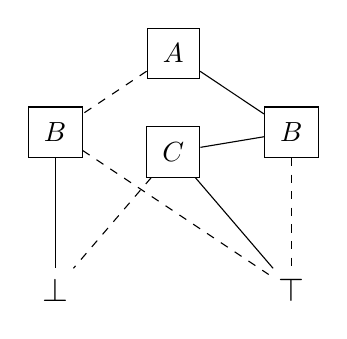
\begin{tikzpicture}
      \node[draw,inner sep=2mm] (a) at (0,0) {$A$};
      \node[draw,inner sep=2mm] (b1) at (-1.5, -1.0) {$B$};
      \node[draw,inner sep=2mm] (b2) at (1.5, -1.0) {$B$};
      \node[draw,inner sep=2mm] (c) at (0.0, -1.25) {$C$};
      \node (F) at (-1.5, -3.0) {\large$\bot$};
      \node (T) at (1.5, -3.0) {\large$\top$};
      \draw[dashed] (a) -- (b1);
      \draw (a) -- (b2);
      \draw[dashed] (b1) -- (T);
      \draw (b1) -- (F);
      \draw[dashed] (b2) -- (T);
      \draw (b2) -- (c);
      \draw[dashed] (c) -- (F);
      \draw (c) -- (T);
    \end{tikzpicture}
  \end{center}
  In their usual notation, inner nodes are variables and leaves are constants $\bot$ and $\top$.
  Evaluating an assignment $\set{x}\in\{0,1\}^n$ is equivalent to a path from the root to a
  leaf where each variable $X$ determines a decision to go through the dashed line when $x=0$ or
  solid line when $x=1$. If the path ends at a $\top$, the function returns 1, otherwise it must
  end at a $\bot$ and therefore returns 0. The BDD above encodes the following logic formula
  \begin{equation*}
    \phi(A,B,C)=(A\vee\neg B)\wedge(\neg B\vee C),
  \end{equation*}
  also shown as a truth table on the right, together with a logic circuit that encodes the same
  truth table and its vtree. Conjunctions take the role of products, with each conjunction node
  determining a vtree node's scope partition.
  \tcblower
  \small%
  \begin{center}
    \begin{tabular}{ccc|c}
      \hline
      $A$ & $B$ & $C$ & $\phi(\set{x})$\\
      \hline
      0 & 0 & 0 & 1\\
      1 & 0 & 0 & 1\\
      0 & 1 & 0 & 0\\
      1 & 1 & 0 & 0\\
      0 & 0 & 1 & 1\\
      1 & 0 & 1 & 1\\
      0 & 1 & 1 & 0\\
      1 & 1 & 1 & 1\\
      \hline
    \end{tabular}

    Truth Table

    \begin{tikzpicture}
      \newOrNode[inputs=nn,fill=boxgreen]{r}{0,0};
      \newAndNode[inputs=nn,fill=boxred!70]{p1}{$(r) + (-1,-1)$};
      \newAndNode[inputs=nn,fill=boxred!70]{p2}{$(r) + (1,-1)$};
      \node (a) at ($(p1) + (-0.5,-1)$) {$A$};
      \newOrNode[inputs=nn,fill=boxpurple!60]{s1}{$(p1) + (0.5,-1)$};
      \node (na) at ($(p2) + (0.5,-1)$) {$\neg A$};
      \newAndNode[inputs=nn,fill=boxblue!80]{q1}{$(s1) + (-0.75,-1)$};
      \newAndNode[inputs=nn,fill=boxblue!80]{q2}{$(s1) + (0.75,-1)$};
      \newAndNode[inputs=nn,fill=boxblue!80]{q3}{$(p2.input 1) + (0,-1.75)$};
      \node (b) at ($(q1) + (-0.5,-1)$) {$B$};
      \node (c1) at ($(q1) + (0.5,-1)$) {$C$};
      \newOrNode[inputs=nn,fill=boxorange!80]{z1}{$(q2.input 1) + (0,-0.75)$};
      \node (nb) at ($(q3.input 2) + (0,-0.75)$) {$\neg B$};
      \node (c) at ($(z1) + (-0.5,-1)$) {$C$};
      \node (nc) at ($(z1) + (0.5,-1)$) {$\neg C$};
      \draw[edge] (r.input 1) -- ++(0,-0.2) -| (p1);
      \draw[edge] (r.input 2) -- ++(0,-0.2) -| (p2);
      \draw[edge] (s1.input 1) -- ++(0,-0.2) -| (q1);
      \draw[edge] (s1.input 2) -- ++(0,-0.2) -| (q2);
      \draw[edge] (p1.input 1) -- ++(0,-0.2) -| (a);
      \draw[edge] (p1.input 2) -- ++(0,-0.2) -| (s1);
      \draw[edge] (p2.input 1) -- (q3);
      \draw[edge] (p2.input 2) -- ++(0,-0.2) -| (na);
      \draw[edge] (q1.input 1) -- ++(0,-0.2) -| (b);
      \draw[edge] (q1.input 2) -- ++(0,-0.2) -| (c1);
      \draw[edge] (q2.input 1) -- (z1.east);
      \draw[edge] (q2.input 2) -- (nb.north);
      \draw[edge] (q3.input 1) -- (z1.east);
      \draw[edge] (q3.input 2) -- (nb.north);
      \draw[edge] (z1.input 1) -- ++(0,-0.2) -| (c);
      \draw[edge] (z1.input 2) -- ++(0,-0.2) -| (nc);
    \end{tikzpicture}

    \vskip -0.25cm
    Equivalent LC

    \begin{tikzpicture}
      \newVtreeNode{r}{0,0}{1};
      \newVtreeNode{l}{$(r) + (0.75,-1)$}{2};
      \newVtreeNode{x1}{$(r) + (-0.75,-1)$}{$A$};
      \newVtreeNode{x2}{$(l) + (-0.75,-1)$}{$B$};
      \newVtreeNode{x3}{$(l) + (0.75,-1)$}{$C$};
      \draw (r) -- (l); \draw (r) -- (x1);
      \draw (l) -- (x2); \draw (l) -- (x3);
    \end{tikzpicture}

    \skip -0.35cm
    Vtree
  \end{center}
\end{example}

\subsection{...to Uncertainty}
\label{subsection:touncertainty}

Logic circuits are easily extensible to probabilistic circuits. In fact, if we think of an LC as
the support of a PC the connections between the two come naturally. Suppose a 2-standard smooth,
structure decomposable and deterministic probabilistic circuit $\mathcal{C}$ over binary variables.
We can construct an identically structured logic circuit (up to input nodes) $\mathcal{L}$ with
same vtree as $\mathcal{C}$ whose underlying Boolean function encodes $\phi(\set{x})=
\left\liv\mathcal{C}(\set{x})>0\right\riv$. Since sums act exactly like disjunctions and products
like conjunctions under the Boolean semiring, products in $\mathcal{C}$ are replaced with
conjunctions in $\mathcal{L}$, and sums with disjunctions. Input nodes from $\mathcal{C}$ are
replaced with a literal node if the function is degenerate, or with a disjunction over positive and
negative literals otherwise. This makes sure $\mathcal{L}$ acts as the support of $\mathcal{C}$, as
each disjunction node $\Sum_{\mathcal{L}}$ of $\mathcal{L}$ defines
\begin{equation*}
  \Sum_\mathcal{L}(\set{x})=\bigvee_{\Child\in\Ch_{\mathcal{C}}(\Sum_\mathcal{L})}\left\liv
  \Child_p(\set{x})>0\right\riv\wedge\left\liv\Child_s(\set{x})>0\right\riv,
\end{equation*}
where $\Ch_{\mathcal{C}}(\Sum)$ retrieves the children of $\Sum$'s corresponding sum node in
$\mathcal{C}$, with $\Child_p(\set{x})$ and $\Child_s(\set{x})$ the probabilities of $\Child$'s
prime and sub respectively. The corresponding sum node $\Sum_{\mathcal{C}}$ in $\mathcal{C}$ then
only attributes a weight (i.e.\ probability) to each positive element as usual
\begin{equation*}
  \Sum_\mathcal{C}(\set{x},\set{y})=\sum_{\Child\in\Ch(\Sum_\mathcal{C})}w_{\Sum_\mathcal{C},\Child}\cdot
  \Child_p(\set{x})\cdot\Child_s(\set{y}).
\end{equation*}
When a deterministic sum (resp. disjunction) node has the above form, then this composition of a
weighted sum (resp. disjunction) is known in PC and LC literature as a \emph{partition}.

\begin{example}[sidebyside,lefthand width=0.55\textwidth]{Embedding certain knowledge in probabilistic circuits}{pcsupp}

  Recall the logic circuit $\mathcal{L}$ from \Cref{eg:bdd}. Imagine we wish to model the
  uncertainty coming from all assignments where $\mathcal{L}(\set{x})=1$. In other words, we want
  to assign a positive probability to all true entries in the previous example's truth table,
  turning it into a probability table. The table on the right shows the chosen probabilities for
  each instance. Naturally, they all sum to one, with logically impossible assignments set to zero.

  Compiling an LC into a PC is straightforward: replace conjunctions with product nodes and
  disjunctions with sum nodes. Input nodes are left untouched, as literal nodes are just degenerate
  probability distributions. Sum weights are what ultimately define the probabilities in the
  probability table. The PC on the right is the result of the compilation of $\mathcal{L}$ into a
  probabilistic circuit whose distribution is defined by the probability table above it. When we
  mean to say that a PC has its support defined by its underlying LC, then we use the logic gate
  notation with the added weights on edges coming out from \inode{\newOrNode} nodes.

  \tcblower
  \small%
  \begin{center}
    \begin{tabular}{ccc|cc}
      \hline
      $A$ & $B$ & $C$ & $\phi(\set{x})$ & $p(\set{x})$\\
      \hline
      0 & 0 & 0 & 1 & 0.140\\
      1 & 0 & 0 & 1 & 0.024\\
      0 & 1 & 0 & 0 & \textcolor{gray}{0.000}\\
      1 & 1 & 0 & 0 & \textcolor{gray}{0.000}\\
      0 & 0 & 1 & 1 & 0.560\\
      1 & 0 & 1 & 1 & 0.096\\
      0 & 1 & 1 & 0 & \textcolor{gray}{0.000}\\
      1 & 1 & 1 & 1 & 0.180\\
      \hline
    \end{tabular}

    Probability Table

    \begin{tikzpicture}
      \newOrNode[inputs=nn,fill=boxgreen]{r}{0,0};
      \newAndNode[inputs=nn,fill=boxred!70]{p1}{$(r) + (-1,-1)$};
      \newAndNode[inputs=nn,fill=boxred!70]{p2}{$(r) + (1.5,-1)$};
      \node (a) at ($(p1) + (-0.5,-1)$) {$A$};
      \newOrNode[inputs=nn,fill=boxpurple!60]{s1}{$(p1) + (0.5,-1.25)$};
      \node (na) at ($(p2) + (0.5,-1)$) {$\neg A$};
      \newAndNode[inputs=nn,fill=boxblue!80]{q1}{$(s1) + (-0.75,-1)$};
      \newAndNode[inputs=nn,fill=boxblue!80]{q2}{$(s1) + (0.75,-1)$};
      \newAndNode[inputs=nn,fill=boxblue!80]{q3}{$(p2.input 1) + (0,-2.0)$};
      \node (b) at ($(q1) + (-0.5,-1)$) {$B$};
      \node (c1) at ($(q1) + (0.5,-1)$) {$C$};
      \newOrNode[inputs=nn,fill=boxorange!80]{z1}{$(q2.input 1) + (0,-1.0)$};
      \node (nb) at ($(q3.input 2) + (0,-1.0)$) {$\neg B$};
      \node (c) at ($(z1) + (-0.5,-1)$) {$C$};
      \node (nc) at ($(z1) + (0.5,-1)$) {$\neg C$};
      \draw[edge] (r.input 1) -- ++(0,-0.2) -| node[near start,above left] {$0.3$} (p1);
      \draw[edge] (r.input 2) -- ++(0,-0.2) -| node[near start,above right] {$0.7$} (p2);
      \draw[edge] (s1.input 1) -- ++(0,-0.2) -| node[near start,above left] {$0.6$} (q1);
      \draw[edge] (s1.input 2) -- ++(0,-0.2) -| node[near start,above right] {$0.4$} (q2);
      \draw[edge] (p1.input 1) -- ++(0,-0.2) -| (a);
      \draw[edge] (p1.input 2) -- ++(0,-0.2) -| (s1);
      \draw[edge] (p2.input 1) -- (q3);
      \draw[edge] (p2.input 2) -- ++(0,-0.2) -| (na);
      \draw[edge] (q1.input 1) -- ++(0,-0.2) -| (b);
      \draw[edge] (q1.input 2) -- ++(0,-0.2) -| (c1);
      \draw[edge] (q2.input 1) -- (z1.east);
      \draw[edge] (q2.input 2) -- (nb.north);
      \draw[edge] (q3.input 1) -- (z1.east);
      \draw[edge] (q3.input 2) -- (nb.north);
      \draw[edge] (z1.input 1) -- ++(0,-0.2) -| node[near start,above left] {$0.8$} (c);
      \draw[edge] (z1.input 2) -- ++(0,-0.2) -| node[near start,above right] {$0.2$} (nc);
    \end{tikzpicture}

    \vskip -0.25cm
    Probabilistic Circuit
  \end{center}
\end{example}

This compatibility between logic and probabilistic circuits allows certain knowledge to be embedded
into an uncertain model by constructing a computational graph whose underlying logic circuit
correctly attributes positive values only to the support of the distribution. When such a
computational graph is also smooth, structure decomposable and deterministic, then it belongs to a
special subclass of PCs called Probabilistic Sentential Decision Diagrams (PSDDs, \cite{kisa14}).
An alternative use case for logic circuits within the context of probabilistic reasoning is
querying for the probability of logical events, i.e.\ the expectation of a logic query with respect
to a distribution. This kind of query is enabled by the following result.

\begin{algorithm}[t]
  \caption{\expc}\label{alg:expc}
  \begin{algorithmic}[1]
    \Require A smooth, structure decomposable PC $\mathcal{C}$ and LC $\mathcal{L}$ both with vtree
      $\vtree$
      \Ensure The expectation $\mathbb{E}_\mathcal{C}\left[\mathcal{L}\right]=\int_\set{x}\mathcal{C}(\set{x})
      \mathcal{L}(\set{x})\dif\set{x}$
    \State Let $v$ be a hash function mapping a pair of nodes to an expectation
    \For{each pair of nodes $(\Node_\mathcal{C},\Node_\mathcal{L})$ in reverse topological order}\label{alg:expc:line:top}
      \IIf{$\Node_\mathcal{C}$ is an input}{$v_{\Node_\mathcal{C},\Node_\mathcal{L}}\gets
        \mathbb{E}_{\Node_\mathcal{C}}\left[\Node_\mathcal{L}\right]$}
      \IElseIf{$\Node_\mathcal{C}$ is a product}{$v_{\Node_\mathcal{C},\Node_\mathcal{L}}\gets
        \prod_{\Child\in\Ch(\Node_\mathcal{C})}v_{\Child_\mathcal{C},\Child_\mathcal{L}}$}
      \IElseIf{$\Node_\mathcal{C}$ is a sum}{$v_{\Node_\mathcal{C},\Node_\mathcal{L}}\gets
        \sum_{\Child'\in\Ch(\Node_\mathcal{C})}\sum_{\Child''\in\Ch(\Node_\mathcal{L})}
        w_{\Sum,\Child'}\cdot v_{\Child',\Child''}$}%
    \EndFor%
    \State \textbf{return} $v_R$, where $\textsf{R}$ is $\mathcal{C}$'s root
  \end{algorithmic}
\end{algorithm}

\begin{restatable}[\cite{choi20}]{theorem}{expcthm}
  If $\mathcal{C}$ is a smooth and structure decomposable probabilistic circuit with vtree
  $\vtree$, and $\mathcal{L}$ a structure decomposable logic circuit also respecting $\vtree$, then
  $\mathbb{E}_\mathcal{C}\left[\mathcal{L}\right]$ is polynomial time computable (in the number of
  edges).
\end{restatable}

Let $\mathcal{C}$ be a smooth and structure decomposable circuit with vtree $\vtree$, and
$\mathcal{L}$ a logic circuit representing a logical query whose vtree is also $\vtree$. Computing
the probability of $\mathcal{L}$ with respect to the distribution encoded by $\mathcal{C}$ is done
by a bottom-up evaluation over both circuits at the same time. \Cref{alg:expc} shows the procedure
algorithmically. Importantly, the procedure relies on evaluating the expectation for each node in
a reverse topological fashion according to line \ref{alg:expc:line:top}. This paired reverse
topological sorting is done by a recursive assignment. For product nodes, primes are paired with
primes, and subs with subs; for sums, each combination of PC child with LC child is paired up.

\begin{example}[sidebyside,lefthand width=0.55\textwidth]{Computing the probability of logical events}{problog}
  \begin{wrapfigure}{r}{0.45\textwidth}
    \centering
    \resizebox{\textwidth}{!}{
    \begin{tikzpicture}
      \newOrNode[inputs=nn,fill=boxgreen]{r}{0,0};
      \newAndNode[inputs=nn,fill=boxred!70]{p1}{$(r) + (-1,-1)$};
      \newAndNode[inputs=nn,fill=boxred!70]{p2}{$(r) + (1,-1)$};
      \node (a) at ($(p1) + (-1,-1)$) {$A$};
      \newOrNode[inputs=nn,fill=boxpurple!60]{s1}{$(p1.input 2) + (0,-0.75)$};
      \node (na) at ($(p2) + (-1,-1)$) {$\neg A$};
      \newOrNode[inputs=nn,fill=boxpurple!60]{s2}{$(p2.input 2) + (0,-0.75)$};
      \newAndNode[inputs=nn,fill=boxblue!80]{q1}{$(s1) + (0,-0.75)$};
      \newAndNode[inputs=nn,fill=boxblue!80]{q2}{$(s2) + (0,-0.75)$};
      \newOrNode[inputs=nn,fill=orange!80]{bb}{$(q1) + (-1,-1)$};
      \newOrNode[inputs=nn,fill=orange!80]{bc1}{$(q1) + (1,-1)$};
      \node (nb) at ($(q2.input 1) + (0,-0.75)$) {$\neg B$};
      \newOrNode[inputs=nn,fill=orange!80]{bc2}{$(q2) + (1,-1)$};
      \node (b1) at ($(bb) + (-0.5,-1)$) {$B$};
      \node (nb1) at ($(bb) + (0.5,-1)$) {$\neg B$};
      \node (c1) at ($(bc1) + (-0.5,-1)$) {$C$};
      \node (nc1) at ($(bc1) + (0.5,-1)$) {$\neg C$};
      \node (c2) at ($(bc2) + (-0.5,-1)$) {$C$};
      \node (nc2) at ($(bc2) + (0.5,-1)$) {$\neg C$};
      \draw[edge] (r.input 1) -- ++(0,-0.2) -| (p1);
      \draw[edge] (r.input 2) -- ++(0,-0.2) -| (p2);
      \draw[edge] (p1.input 1) -- ++(0,-0.2) -| (a);
      \draw[edge] (p2.input 1) -- ++(0,-0.2) -| (na);
      \draw[edge] (p1.input 2) -- (s1);
      \draw[edge] (p2.input 2) -- (s2);
      \draw[edge] (s1) -- (q1);
      \draw[edge] (s2) -- (q2);
      \draw[edge] (q1.input 1) -- ++(0,-0.2) -| (bb);
      \draw[edge] (q1.input 2) -- ++(0,-0.2) -| (bc1);
      \draw[edge] (q2.input 1) -- (nb);
      \draw[edge] (q2.input 2) -- ++(0,-0.2) -| (bc2);
      \draw[edge] (bb.input 1) -- ++(0,-0.2) -| (b1);
      \draw[edge] (bb.input 2) -- ++(0,-0.2) -| (nb1);
      \draw[edge] (bc1.input 1) -- ++(0,-0.2) -| (c1);
      \draw[edge] (bc1.input 2) -- ++(0,-0.2) -| (nc1);
      \draw[edge] (bc2.input 1) -- ++(0,-0.2) -| (c2);
      \draw[edge] (bc2.input 2) -- ++(0,-0.2) -| (nc2);
    \end{tikzpicture}
    }
  \end{wrapfigure}
  Say we have a PC encoding the distribution shown in the table on the right. Suppose we wish to
  compute the probability of a logical event, say $\phi\equiv A\vee\neg B$. A naïve approach would
  be to go over each assignment $\set{x}$ where $\phi(\set{x})=1$, and compute their sum. This is
  obviously exponential on the number of variables. Instead, we may compile $\phi$ into the logic
  circuit above and run the \expc{} algorithm to (in polynomial time) compute this otherwise
  intractable marginalization. Running the \expc{} gives us a probability of
  $0.6415=1.0-(0.1365+0.2220)$, which is exactly the desired probability.
\tcblower
\begin{center}
  \resizebox{\textwidth}{!}{
  \begin{tikzpicture}
    \newOrNode[inputs=nn,fill=boxgreen]{r}{0,0};
    \newAndNode[inputs=nn,fill=boxred!70]{p1}{$(r) + (-1,-1)$};
    \newAndNode[inputs=nn,fill=boxred!70]{p2}{$(r) + (1,-1)$};
    \newOrNode[inputs=nn,fill=boxpurple!60]{ba1}{$(p1) + (-1.5,-1)$};
    \newOrNode[inputs=nn,fill=boxpurple!60]{s1}{$(p1.input 2) + (0.0,-0.75)$};
    \newOrNode[inputs=nn,fill=boxpurple!60]{s2}{$(p2.input 1) + (0.0,-0.75)$};
    \newOrNode[inputs=nn,fill=boxpurple!60]{ba2}{$(p2) + (1.5,-1)$};
    \node (a1) at ($(ba1) + (-0.75,-1)$) {$A$};
    \node (na1) at ($(ba1.input 2) + (0.0,-0.75)$) {$\neg A$};
    \newAndNode[inputs=nn,fill=boxblue!80]{q1}{$(s1.input 1) + (0,-0.75)$};
    \newAndNode[inputs=nn,fill=boxblue!80]{q2}{$(s2.input 2) + (0,-0.75)$};
    \node (a2) at ($(ba2.input 1) + (0.0,-0.75)$) {$A$};
    \node (na2) at ($(ba2) + (0.75,-1)$) {$\neg A$};
    \newOrNode[inputs=nn,fill=orange!80]{bb1}{$(q1) + (-1.5,-1)$};
    \newOrNode[inputs=nn,fill=orange!80]{bc1}{$(q1.input 2) + (0,-0.75)$};
    \newOrNode[inputs=nn,fill=orange!80]{bb2}{$(q2.input 1) + (0,-0.75)$};
    \newOrNode[inputs=nn,fill=orange!80]{bc2}{$(q2) + (1.5,-1)$};
    \node (b1) at ($(bb1) + (-0.75,-1)$) {$B$};
    \node (nb1) at ($(bb1.input 2) + (0.0,-0.75)$) {$\neg B$};
    \node (c1) at ($(bc1) + (-0.5,-1)$) {$C$};
    \node (nc1) at ($(bc1) + (0.5,-1)$) {$\neg C$};
    \node (b2) at ($(bb2) + (-0.5,-1)$) {$B$};
    \node (nb2) at ($(bb2) + (0.5,-1)$) {$\neg B$};
    \node (c2) at ($(bc2.input 1) + (0.0,-0.75)$) {$C$};
    \node (nc2) at ($(bc2) + (0.75,-1)$) {$\neg C$};
    \draw[edge] (r.input 1) -- ++(0,-0.2) -| node[near start,above left] {$.45$} (p1);
    \draw[edge] (r.input 2) -- ++(0,-0.2) -| node[near start,above right] {$.55$} (p2);
    \draw[edge] (p1.input 1) -- ++(0,-0.2) -| (ba1);
    \draw[edge] (ba1.input 1) -- ++(0,-0.2) -| node[near start, above left] {$.7$} (a1);
    \draw[edge] (ba1.input 2) -- node[midway, right] {$.3$} (na1);
    \draw[edge] (p2.input 2) -- ++(0,-0.2) -| (ba2);
    \draw[edge] (ba2.input 1) -- node[midway, left] {$.6$} (a2);
    \draw[edge] (ba2.input 2) -- ++(0,-0.2) -| node[near start, above right] {$.4$} (na2);
    \draw[edge] (p1.input 2) -- ++(0,-0.2) -| (s1);
    \draw[edge] (p2.input 1) -- ++(0,-0.2) -| (s2);
    \draw[edge] (s1.input 1) -- node[midway,left] {$.2$} (q1.east);
    \draw[edge] (s1.input 2) -- node[near start,above right,xshift=-0.1cm] {$.8$} (q2.east);
    \draw[edge] (s2.input 1) -- node[near start,above left,xshift=0.1cm] {$.9$} (q1.east);
    \draw[edge] (s2.input 2) -- node[midway,right] {$.1$} (q2.east);
    \draw[edge] (q1.input 1) -- ++(0,-0.2) -| (bb1);
    \draw[edge] (q1.input 2) -- ++(0,-0.2) -| (bc1);
    \draw[edge] (q2.input 1) -- ++(0,-0.2) -| (bb2);
    \draw[edge] (q2.input 2) -- ++(0,-0.2) -| (bc2);
    \draw[edge] (bb1.input 1) -- ++(0,-0.2) -| node[near start,above left] {$.4$} (b1);
    \draw[edge] (bb1.input 2) -- node[midway,right] {$.6$} (nb1);
    \draw[edge] (bc1.input 1) -- ++(0,-0.2) -| node[near start,above left] {$.5$} (c1);
    \draw[edge] (bc1.input 2) -- ++(0,-0.2) -| node[near start,above right] {$.5$} (nc1);
    \draw[edge] (bb2.input 1) -- ++(0,-0.2) -| node[near start,above left] {$.5$} (b2);
    \draw[edge] (bb2.input 2) -- ++(0,-0.2) -| node[near start,above right] {$.5$} (nb2);
    \draw[edge] (bc2.input 1) -- node[midway, left] {$.2$} (c2);
    \draw[edge] (bc2.input 2) -- ++(0,-0.2) -| node[near start,above right] {$.8$} (nc2);
  \end{tikzpicture}
  }

  \begin{tabular}{ccc|cc}
    \hline
    $A$ & $B$ & $C$ & $\phi(\set{x})$ & $p(\set{x})$\\
    \hline
    0 & 0 & 0 & 1 & .1000\\
    1 & 0 & 0 & 1 & .0580\\
    0 & 1 & 0 & 0 & \textcolor{gray}{.1365}\\
    1 & 1 & 0 & 1 & .0805\\
    0 & 0 & 1 & 1 & .1860\\
    1 & 0 & 1 & 1 & .0970\\
    0 & 1 & 1 & 0 & \textcolor{gray}{.2220}\\
    1 & 1 & 1 & 1 & .1195\\
    \hline
  \end{tabular}
\end{center}
\end{example}

\begin{remark}[breakable]{On applications of probabilistic circuits}{applications}
  So far, we have not yet addressed real-world applications of probabilistic circuits. Although
  their usage has not yet gained popularity among the data science crowd, they have been
  successfuly employed in a multitude of interdisciplinary tasks. Here, we give a brief survey on
  the different use cases of probabilistic circuits present in literature.

  Computer vision is perhaps the most popular application for deep learning, and this could not be
  different for probabilistic circuits. PCs have been used for image classification
  \citep{gens12,sguerra16,llerena17,geh19,peharz20a}, image reconstruction and sampling
  \citep{poon11,dennis17,peharz20b,butz19}, image segmentation and scene understanding
  \citep{friesen17,yuan16,friesen18,rathke17}, and activity recognition
  \citep{wang18,amer12,nourani20,amer16}.

  Probabilistic circuits have also been used for sequential data \citep{melibari16b}, such as
  speech recognition and reconstruction \citep{peharz14b,ratajczak14,ratajczak18} and natural
  language processing \citep{cheng14}.

  Remarkably, probabilistic circuits have seen a recent boom in hardware-aware research
  \citep{shah19,olascoaga19} and dedicated hardware for PCs in embedded systems
  \citep{sommer18,shah20,shah21}.

  Some other applications include robotics \citep{sguerra16,geh19,zheng18,pronobis17}, biology
  \citep{butz18,friesen15}, probabilistic programming \citep{stuhlmuller12,saad21}, and fault
  localization \citep{nath16}.
\end{remark}

Now that we have addressed the (arguably) most important aspects of probabilistic circuits, we are
now ready to understand how to build them in a principled way.

